\documentclass[10pt,1p,authoryear]{elsarticle}
\usepackage[utf8]{inputenc}

\setlength{\tabcolsep}{1.3pt}
\setlength{\columnsep}{0.4cm}
\usepackage{acronym}
\usepackage{amsmath}
\usepackage{amssymb}
\usepackage{array}
\usepackage{bm}
\usepackage{booktabs}
\usepackage[aboveskip=1pt,labelfont=bf,labelsep=period,justification=raggedright,singlelinecheck=off, font=small]{caption}
\usepackage{diagbox}
\usepackage{float}
\usepackage[T1]{fontenc}
% \usepackage[a4paper,inner=2cm,outer=2cm,top=2.5cm,bottom=2.5cm]{geometry}
\usepackage{graphicx}% Include figure files
\usepackage{here}
\usepackage{hyperref}
%\usepackage{lipsum}
\usepackage{lineno}
\usepackage{setspace}
\usepackage{mathtools}
\usepackage{mathrsfs}
\usepackage{multirow}
\usepackage{newfloat}
\usepackage{onimage}
\usepackage{siunitx}
\usepackage{subcaption}
\usepackage{tabularx}
\usepackage{tikz}
%\usepackage[dvipsnames]{xcolor}
\usepackage{xpatch}
\usepackage{orcidlink}

% Ensure that subcaptions have capital letter
\renewcommand{\thesubfigure}{\Alph{subfigure}}

% Must be loaded after tikz
\usepackage{ctable}

% Define new column type with multirow
\newcolumntype{M}[1]{>{\centering\arraybackslash}m{#1}}

\bibliographystyle{elsarticle-harv}

\restylefloat{table}

% Remove indent across the whole document
\setlength\parindent{0pt}

% Define equation numbering
\numberwithin{equation}{section}


\newcommand{\mbx}{\mathbf{x}}
\newcommand{\mbm}{\mathbf{m}}
\newcommand{\mbp}{\mathbf{p}}
\newcommand{\mbu}{\mathbf{u}}
\newcommand{\mbF}{\mathbf{F}}
\newcommand{\mbH}{\mathbf{H}}
\newcommand{\cmt}[1]{\textcolor{red} {[#1]}}
\newcommand{\etal}{{\textit{et al. }}}

\newacro{ode}[ODE]{Ordinary Differential Equation}
\newacro{pde}[PDE]{Partial Differential Equation}
\newacro{glv}[gLV]{generalized Lotka-Volterra}
\newacro{abm}[ABM]{Agent-Based Model}


% Define new style for json listings
% Copied from https://www.latex4technics.com/?note=3QTU
\colorlet{punct}{red!60!black}
\definecolor{background}{HTML}{EEEEEE}
\definecolor{delim}{RGB}{20,105,176}
\colorlet{numb}{magenta!60!black}

\title{The Pool Model: A Mechanistic ODE Framework for Bacterial Consortia in Food Science}
\author[1]{Polina Gaindrik\orcidlink{0000-0003-0928-3951}}
\author[1]{Jonas Pleyer\orcidlink{0009-0001-0613-7978}}
\author[2]{Matthias Brunner}
\author[3]{Fernando Pérez Rodríguez}
\author[1]{Christian Fleck\orcidlink{0000-0002-6371-4495}\corref{cor1}}
\ead{christian.fleck@fdm.uni-freiburg.de}

\cortext[cor1]{Corresponding Author\\ \textit{E-mail address:} christian.fleck@fdm.uni-freiburg.de}
\affiliation[1]{
    organization={Freiburg Center for Data Analysis and Modeling and AI},
    addressline={Ernst-Zermelo Str. 1},
    city={Freiburg im Breisgau},
    postcode={79104},
    country={Germany},
}
\affiliation[2]{
    organization={tsenso GmbH},
    addressline={Nöllenstr. 32},
    city={Stuttgart},
    postcode={70195},
    country={Germany},
}
\affiliation[3]{
    organization={Department of Food Science and Technology, UIC Zoonosis y Enfermedades Emergentes ENZOEM, ceiA3, Universidad de Córdoba},
    addressline={Campus Rabanales s/n. Darwin building- Annex},
    city={Córdoba},
    postcode={14014},
    country={Spain},
}
\date{
    \footnotesize
    \textsuperscript{\textbf{1}}
}

% Force double spacing in abstract (elsarticle overrides \doublespacing there)
\makeatletter
\let\els@abstract\abstract
\renewcommand{\abstract}{\els@abstract\setstretch{2}}
\makeatother

\begin{document}
\doublespacing
\linenumbers

\begin{abstract}
Predictive microbiology in food science requires models that are both mechanistically
interpretable and flexible enough to describe the diversity of bacterial behaviors in
complex food matrices. We introduce the pool model, an \ac{ode}-based framework in which bacterial populations
are partitioned into discrete metabolic states -- pools -- with biologically motivated
transitions between them. The framework systematically incorporates single-cell processes such as lag phase
adaptation, growth, death, and dormancy, and extends naturally to multi-species consortia. For a single species, the three-pool model with a limiting resource reproduces the
characteristic sigmoidal growth curve. A dormancy extension based on a Maxwell-type
stress-strain relation captures the experimentally observed asymmetric response of
bacteria to temperature shifts. For two-species systems, the framework encompasses resource competition, which
reduces exactly to the generalized Lotka-Volterra equations as a special case, as
well as toxin production, mutual inhibition, and mutualism. To assess the validity of the \ac{ode} approximation, we derive the pool model
analytically from an \ac{abm}, demonstrating that it arises naturally from individual
cell-level behavior. Numerical comparisons across four spatial configurations show that the \ac{ode}
description holds in the well-mixed limit with fast nutrient diffusion, while spatial
heterogeneity and slow diffusion introduce systematic deviations in the predicted
growth curves. The pool model thus provides a unified, mechanistically interpretable starting point
for modeling bacterial consortia in food safety applications.
\end{abstract}

%%Graphical abstract
%\begin{graphicalabstract}
%\includegraphics{grabs}
%\end{graphicalabstract}

\begin{highlights}
    \item Pool model framework partitions bacterial populations into discrete metabolic states
    \item Lag phase, dormancy, death, and resource dependence are incorporated systematically
    \item Dormancy via Maxwell stress-strain relation captures asymmetric temperature response
    \item Resource competition reduces exactly to the generalized Lotka-Volterra equations
    \item Toxin production, mutual inhibition, and mutualism extend the two-species framework
\end{highlights}

\begin{keyword}
    Bacterial Consortia
    \sep Competition and Cooperation
    \sep Mechanistic Modeling
    \sep Spatial Effects
    \sep Predictive Modeling
\end{keyword}

\maketitle
%
% ================================================================================================
\section{Introduction}
Bacterial consortia are highly complex systems that consist of multiple distinct cell types.
The underlying processes are interconnected and occur on all scales, ranging from
population-based dynamics of colony growth through molecular processes such as metabolism to gene
expression. In particular, food matrices represent highly relevant and complex microbial ecosystems, where these communities
play a key role in both food safety and spoilage as well as fermentation processes.
In this domain, biofilms represent an important source of contamination and an increased risk of infection. These biological structures are formed by complex and dynamic microbial communities that adhere to
surfaces, develop various communication mechanisms (e.g., quorum sensing), and coordinate to
improve nutrient accessibility and provide protection against antimicrobial chemicals and physical
stress~\citep{Zhao2023}.\\
%
Due to their enormous practical importance, bacterial systems have been studied in detail. 
During the growth process, bacteria undergo different physiological and metabolic
states~\citep{buchanan_when_1997} that determine growth dynamics and response to the environment.
Typically, when bacteria colonize a new environment, they enter an adaptation phase, commonly
referred to as lag time~\citep{monod_growth_1949, swinnen_predictive_2004, rolfe_lag_2012}.
During this phase, bacteria prepare the enzymatic and metabolic machinery to initiate cell division
and multiplication.
According to \cite{baranyi_dynamic_1994}, lag time can be defined as a function of the concentration of a limiting component that cells must synthesize
to start growing. Additionally, bacteria can cooperate, e.g., via complementary metabolic processes, or inhibit
each other, e.g., by means of waste production as a metabolic byproduct~\citep{west_social_2007, rainey_evolution_2003, hibbing_bacterial_2010, stubbendieck_bacterial_2016}. A food-relevant example is the inhibition of \textit{Listeria monocytogenes} by bacteriocin-producing lactic acid bacteria in fermented meat and dairy products~\citep{cotterBacteriocinsDeveloping2005, rileyBacteriocinsEvolution2002}.
A limited supply of nutrients will also affect the overall reproductive capacity of the colony~\citep{monod_growth_1949}.
Bacteria have thus devised various survival strategies to ensure sufficient access to nutrients. Effects at the single-cell level, such as adhesion~\citep{htuson_bacteriasurface_2013}, migration~\citep{decoene_microscopic_2011}, and chemotaxis, can lead to complex phenomena at the population level that contribute to colony survival.

Cell signaling, e.g., in the form of quorum-sensing, can lead to collective emergent phenomena such as
biofilm formation that play an important role in many mature microbial communities~\citep{Jin2020,ng_bacterial_2009}.\\
%
The first step in the construction of any mathematical model is to determine the required level of
detail with respect to the description scale and consequently which effects to include.
Bacterial growth curves allow us to describe the dynamics of overall species abundance. The field of predictive microbiology has developed a variety of ordinary differential equation (ODE)-based models to
capture bacterial growth dynamics~\citep{perez-rodriguez_predictive_2012, gaindrik_experimental_2025}.
Various \ac{ode} \textit{primary models} describe the bacterial growth curve under constant
environmental conditions.
Widely used examples include the modified Gompertz model~\citep{Zwietering1990,Gompertz1825-wi,Gibson1987}, Baranyi-Roberts
model~\citep{baranyi_modeling_1993, baranyi_dynamic_1994}, and the two-compartment model~\citep{McKellar1997} that distinguishes between growing and non-growing bacteria~\citep{buchanan_when_1997}. To take into account changing environmental conditions, so-called \textit{secondary models}
express the model parameters as a function of external quantities such as temperature, pH, or
humidity. Temperature fluctuations during cold-chain interruptions represent a particularly relevant scenario in food storage and transport, where
dormancy transitions directly affect pathogen growth dynamics~\citep{swinnen_predictive_2004}.
Secondary models can be simple polynomial models, square root-type models~\citep{ratkowsky_relationship_1982}, or
more complex relations such as the cardinal parameter model~\citep{zwietering_decision_1992}.
The advantage of the \ac{ode} formulation lies in the predictive power and ease of use.
However, due to their coarse-grained nature, they lack the ability to describe heterogeneity and
other spatial effects.\\
%
When dealing with spatial effects such as heterogeneity, one is required to use more extensive
modeling formulations such as \acp{pde} or \acp{abm}. Such heterogeneity is characteristic of structured food matrices, including soft cheeses, minced meat products, and biofilms on food-contact surfaces~\citep{cauchie_modeling_2020, mounier_microbial_2008}.
\acp{pde} represent an intermediate step between the population-based \ac{ode} models and the
individual-based \acp{abm} and can be effective, especially when dealing with large populations of
cells that can be approximated as a continuum.
On the other hand, \acp{abm} excel at describing the individual behavior of cells that can then lead to more complex collective phenomena.
Tools such as BSim~\citep{Gorochowski2012,Dang2020}, AgentCell~\citep{emonet_agentcell_2005}, BacSim~\citep{kreft_bacsim_1998}, or \texttt{cellular\_raza}~\citep{Pleyer2025} are
capable of describing large numbers of bacteria, performing various intracellular and extracellular
processes. The latter has been used to adapt \ac{pde}-based models into an \ac{abm} formulation that describes
bacterial branching patterns~\citep{Kawasaki1997,Matsushita1998}.\\
%
In this work, we introduce a new \ac{ode}-based modeling framework that describes various
bacterial species, their metabolic states, and external quantities such as nutrients as individual pools.
The dynamics of bacterial growth can be understood in terms of transitions between the different
bacterial states, i.e., pools. Our model allows us to capture interactions between these bacterial states and the external
microenvironment. Compared with the aforementioned methods, this approach turns out to be less complex with general
applicability, a low number of parameters, and greater interpretability of the underlying biology.
To illustrate the generality of the model, multiple examples are reported. We analyze the spatial limitations of an interacting two-species model and show that it can be fully
understood on an individual-based level in terms of single-cell processes. Furthermore, we assess how spatial heterogeneity~\citep{mckellar_heterogeneous_1997} can impact the shape of the growth curves.
%
% ================================================================================================
\section{One species modeling}
% ------------------------------------------------------------------------------------------------
\subsection{Three-pool model}
\label{sec:three-pool-model}
We begin our analysis by considering a simple system where only one species is present. Bacteria undergo different consecutive growth phases~\citep{buchanan_when_1997}, starting with the lag phase, which is a specific case of quiescence, during which no increase in the bacterial count occurs. This quiescent period arises from the microbial community's need to adapt, for example, to the new environmental conditions. This so-called preparation before the exponential growth includes synthesis of the necessary compounds, initiation of transcription~\citep{rolfe_lag_2012}, and other physiological and regulatory mechanisms~\citep{monod_growth_1949}. After this, the bacteria that have succeeded in this adaptation stage enter the exponential growth phase, where the process of cell division is predominant. When nutrient levels are exhausted by the growing bacteria, the stationary state of the growth curve occurs. In this state, the cultures accumulate waste products of metabolic activity that lead to cell death in the bacterial colony. At the same time, dying cells release the nutrients for survivors to continue growing. As a result, the balance between the growing and dying processes leads to a constant bacterial count~\citep{navarro_llorens_stationary_2010}. In the described simplified version of the real-life system, three distinct bacterial states can be identified, corresponding to the underlying processes: adaptation, growth, or death. Motivated by this, we divide a bacterial population into three pools (states) (Figure~\ref{fig:SchematicRep}), defining the fraction of the population in the lag phase $L(t)$, growing and dividing $G(t)$, and undergoing cell death $D(t)$.
\begin{figure}[H]
    \begin{center}
    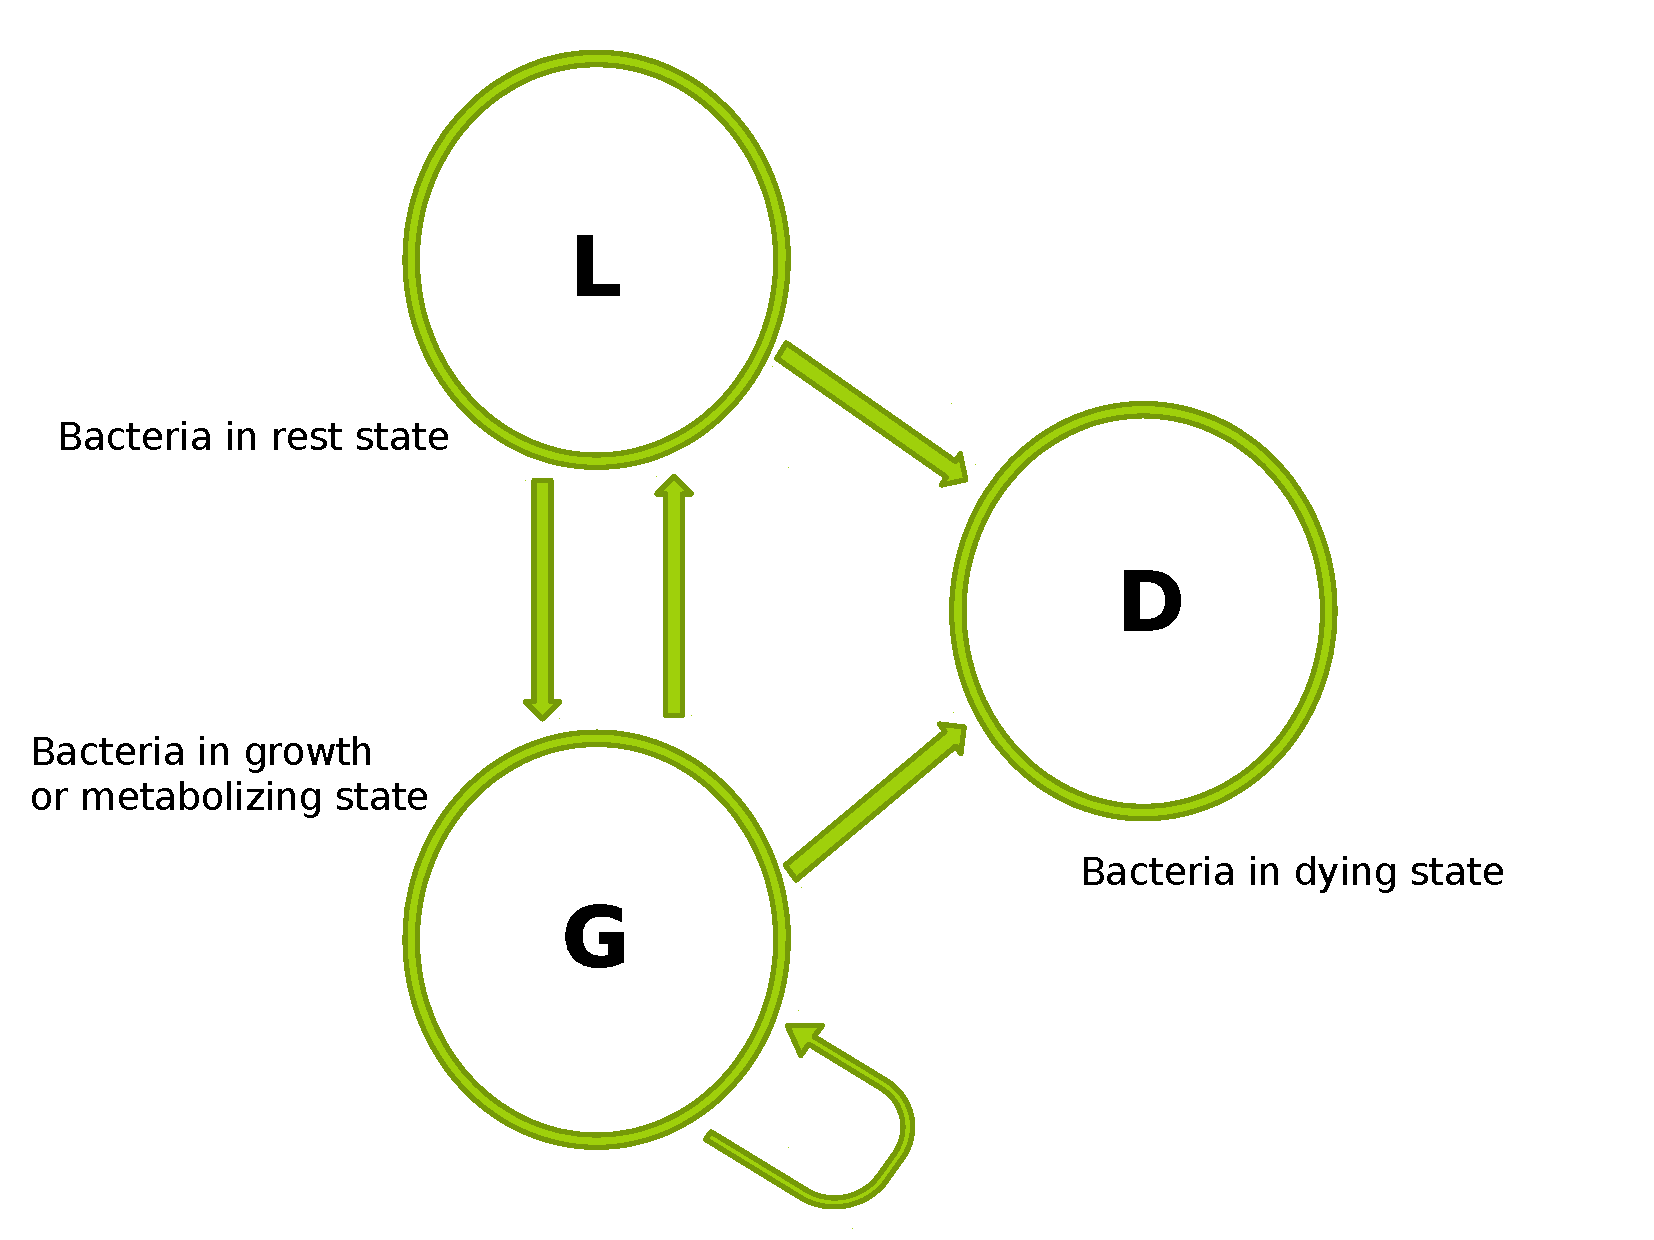
\includegraphics[width=0.95\columnwidth]{Figures-TPM_fig.pdf}
    \caption{Schematic representation of exchange between three states or pools.}
    \label{fig:SchematicRep}
    \end{center}
\end{figure}
To determine the equations that describe the system's dynamics, we consider the flows between the different states.
The pools $G$ and $D$ are unidirectionally connected to the pool $L$. For now, we assume no backflow from the growth state $G$ to the lag-state $L$.
This is a reasonable assumption for conditions that remain constant. The proposed model can be cast in the following reactions:
\begin{align}
\begin{split}
    L &\stackrel{\lambda}{\longrightarrow} G\\
    L &\stackrel{\omega}{\longrightarrow} D\\
    G &\stackrel{\mu}{\longrightarrow} 2G\\
    G &\stackrel{\omega'}{\longrightarrow} D.
\end{split}
\end{align}
Then the \acp{ode} describing such a model can be written as
\begin{align}\begin{split}
    \dot{L} &= -(\omega + \lambda) L\\
    \dot{G} &= \lambda L + \mu G - \omega' G\\
    \dot{D} &= \omega  L + \omega' G,
\end{split}\end{align}
with the initial conditions $L(0)=N_0$, $G(0)=0$, and $D(0)=0$, where $N_0$ is the initial bacterial population.
%

\subsection{Dependence on external resources}
Experimental observations have shown that the bacterial growth is strongly influenced by the limiting resource.
According to the works of \citet{monod_growth_1949} and \citet{vanimpeNovelClass2005}, in the system where all needed nutrients are in excess except for one, the total growth is proportional to the concentration of this limiting nutrient resource.
% The control of the population density with respect to the available nutrition by means of cell communication is called quorum sensing.
We choose a minimal approach to describe the dependence of growth on the nutrient availability.
We include a resource pool that is consumed by the growing bacteria using the second-order kinetic reaction:
\begin{equation}
    G + R  \stackrel{\mu_0}{\longrightarrow} 2G,
\end{equation}
allowing us to keep a minimal number of parameters.
Note that the pools $L$, $G$, and $D$ represent the number of bacteria (or number of bacteria per unit area/volume) while $R$ represents an abstract resource pool. $R=N_R/V$ and $[R]=1/V$, where $N_R$ is the number of resource molecules (or any appropriate unit, e.g., \unit{mol}).
Then $[\mu_0]=\unit{V/h}$, $[N_t]=1/V$, and $[\mu]= 1/h$.
$N_t$ denotes the maximal size of the total bacterial population due to environmental limitations. For simplicity, we introduce the constant $\mu:=\mu_0 N_t$ and the dimensionless resource pool $\tilde{R}(t) = R/ N_t$ ($0 \leqslant \tilde{R}(t) \leqslant 1, \, \forall t$).
Here the full capacity of the resource pool $N_t$ was used as a scaling constant.
In this case the growth term can be simply written as $\mu G \tilde{R}$ and the model is fully formulated in the following way:
\begin{align}
    \begin{split}
        \dot{L} &= -(\omega + \lambda) L\\
        \dot{G} &= \lambda L + \mu \tilde{R} G-\omega' G\\
        \dot{D} &= \omega  L + \omega' G\\
        \dot{\tilde{R}} &= - \frac{\mu}{N_t} \tilde{R} G.
    \end{split}
\label{eq:ode_3pool_resource}
\end{align}
%
This can be simplified by exploiting the conservation of the resource pool:
\begin{equation}
    \tilde{R} = 1 - \frac{L+G+D}{N_t}, 
\end{equation}
and, hence, the full system can be written as:
\begin{align}
    \begin{split}
        \dot{L} &= -(\omega + \lambda) L\\
        \dot{G} &= \lambda L + \mu G\left(1-\frac{L+G+D}{N_t}\right)-\omega' G\\
        \dot{D} &= \omega  L + \omega' G.
    \end{split}
\label{eq:ode_3pool_resource2}
\end{align}
%
%
\begin{figure}[H]
    \begin{center}
    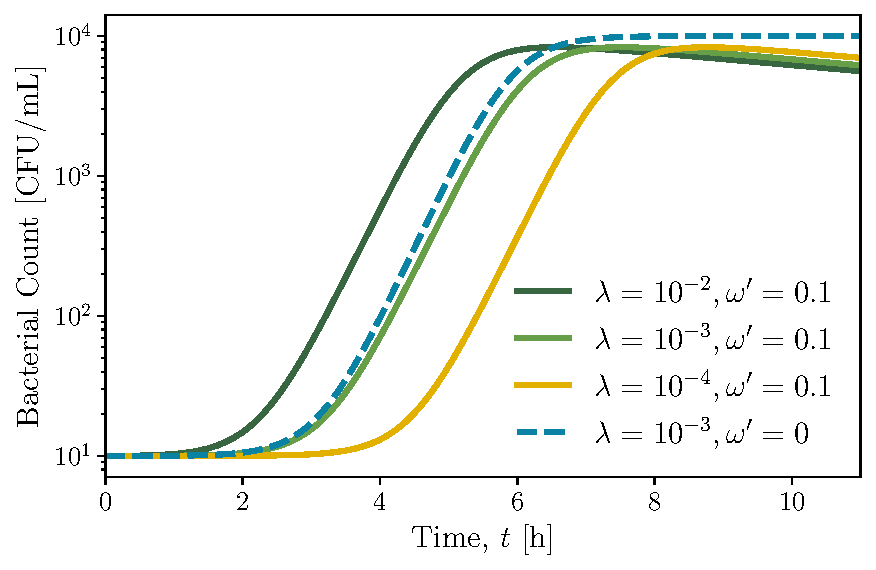
\includegraphics[width=0.9\columnwidth]{Figures-pool_model_3pools_resource.pdf}
    \caption{
        The time dependence of the bacterial count $L(t) + G(t) $ is shown calculated using the model (\ref{eq:ode_3pool_resource2}) with parameters $\mu=2.5~\mathrm{h}^{-1}$, $\omega=0~\mathrm{h}^{-1}$, $N_t = 10^4$,  $N_0 = 10$.
        The blue dashed curve shows the case of no cell death $\omega' = 0~\mathrm{h}^{-1}$ and thus exhibits a steady state without the decrease of the bacterial population.
        Other curves represent the growing bacteria dying with the rate $\omega'=0.1~\mathrm{h}^{-1}$ and different lengths of lag phases: short $\lambda=10^{-2}~\mathrm{h}^{-1}$ (dark green), intermediate $\lambda=10^{-3}~\mathrm{h}^{-1}$ (light green), and a long one $\lambda=10^{-4}~\mathrm{h}^{-1}$ (yellow).
        Note that the steady state for $L(t)+G(t)$ and $D(t)$ is for this model $\lim_{t\to\infty} L(t)+G(t)=0$ and $\lim_{t\to\infty} D(t)=N_t$.
    }
    \label{fig:3pool_resource_plots}
    \end{center}
\end{figure}
The resulting growth curves for the three-pool case are presented in Figure~\ref{fig:3pool_resource_plots}.
The value of the transition rate $\lambda$ determines the duration of the lag phase.
The larger this rate is, the shorter the lag time. Moreover, by including the flow of living bacteria to the death pool, we can model a greater variety of effects by allowing a decrease in the bacterial count.
%
% ------------------------------------------------------------------------------------------------
\subsection{Lag time estimation}
Note that the previously introduced model could be further simplified to a two-pool model by omitting the pool $D$ and removing cells directly from pools $L$ and $G$.
The relevant question here is whether cells in the pool $D$ have any significant impact on resource availability, e.g., by freeing previously occupied spaces or releasing previously consumed nutrients.
If yes, the three-pool model would be advantageous, if not, the two-pool model is sufficient with the benefit of having one fewer parameter.\\
%
The dynamics of the three-pool model are captured by equations~(\ref{eq:ode_3pool_resource2}) that can be used to derive the two-pool model simply by omitting $D$.
Moreover, for $\omega'=0$ the equations for $L$ and $D$ can be readily integrated resulting in:
\begin{align}
    \begin{split}
        L(t) &= N_0 e^{-(\omega+\lambda)t}\\
        D(t) &= N_0 \omega \frac{1-e^{-(\omega+\lambda)t}}{\omega+\lambda
       }.
    \end{split}
\end{align}
For constant parameters $\omega$ and $\lambda$, the integrals for $L$ and $D$ can be inserted into the differential equation for $G$.
However, in the case of time-dependent parameters, e.g., for a dependence on a non-static, dynamic temperature, it is not advantageous to use the analytical results for $L$ and $D$; instead one should work with all three equations for $L$, $G$, and $D$.
It is interesting to see what type of equations result for the total bacterial population $\mathcal{N}=L+G+D$:
\begin{align}
    \begin{split}
        \dot{G} &= \lambda L + \mu G\left(1-\frac{\mathcal{N}}{N_t}\right)\\
        \dot{\mathcal{N}} &= \mu G\left(1-\frac{\mathcal{N}}{N_t}\right),
    \end{split}
\end{align}
with initial conditions $G(0)=0$ and $\mathcal{N}(0)=N_0$.
These equations have a clear interpretation, are derived from first principles, and are not identical to the popular Baranyi-Roberts and modified-Gompertz models.
A notable difference is that the growth rate $\mu$ is time-independent.
For the functions $L$ and $D$ it holds: $\lim_{t\to\infty} L(t) = 0$ and  $\lim_{t\to\infty} D(t) =  N_0\frac{\omega}{\omega+\lambda} $.
It follows immediately that $\lim_{t\to\infty} G(t) = N_t-N_0\frac{\omega}{\omega+\lambda}$.
The lag time $t_L$ can be approximated by the time at which half of the initial population is in the growth phase, i.e., $N_0=2G(t_L)$.
This approach differs from other concepts of lag time such as the one by Gompertz (geometric lag time) or Baranyi (time of adjustment).

Assuming $L\ll N_t$, we can ignore the non-linear term in the equation for $G$, which gives rise to:
\begin{align}
    N_0&= 2\int_0^{t_L} \lambda L(t)e^{\mu(t_L-t)}dt\\
    1  &= 2\lambda e^{\mu t_L}\frac{1-e^{-(\omega+\lambda+\mu)t_L}}{\omega+\lambda+\mu}.
\end{align}
For $\mu > \omega+\lambda$  we can approximate $t_L$ by:
\begin{align}
    t_L &\approx -\frac{1}{\mu}\ln\left(\frac{2\lambda}{\omega+\lambda+\mu}\right).
\end{align}
The lag time $t_L$ diverges very slowly, logarithmically, with $\lambda\to 0$.
%
%
% ------------------------------------------------------------------------------------------------
\subsection{Dormancy}
To demonstrate the flexibility of the proposed modeling approach, we consider the transition from the growth to the dormant state. Bacteria that have lived under unfavorable conditions have developed different survival mechanisms, one of which involves adapting their metabolism and transitioning into a dormant state. 
Dormancy in bacteria is a reversible state in which cells maintain low metabolic activity while cell division ceases~\citep{kaprelyants_dormancy_1993}.
This survival strategy can arise in response to various external stresses, e.g., nutrient deficiency, temperature stress, or extreme fluctuations in microenvironmental parameters.
Having survived periods of stress, bacteria can continue growing and dividing~\citep{kell_viability_1998}.
A variety of models that include transitions of bacteria to the dormant state were proposed by \citet{bar_modelling_2002} and \citet{jones_dormancy_2010}.
%
We now aim to investigate the case where parts of the population $G$ enter a dormant state under stress conditions.
Within the framework of the pool model, we define a new metabolic state $S$ corresponding to the bacterial stress:
\begin{align}
\begin{split}
    L &\stackrel{\lambda}{\longrightarrow} G\\
    G+R &\stackrel{\mu_0}{\longrightarrow} 2G\\
    G &\stackrel{\omega'}{\longrightarrow} D\\
    G &\stackrel{\gamma(t)}{\longrightarrow} S\\
    S &\stackrel{\xi}{\longrightarrow} G.
    \end{split}
\end{align}
We set $\omega=0$ for simplicity. The transition rate of the growing bacteria to the stress state $\gamma(t)$ depends on the change of the environment.
Stronger and more rapid changes will lead to a higher rate $\gamma$, but the effect will relax to zero after some time~\citep{lennon_microbial_2011}.
After the extreme conditions are overcome, the bacteria return to normal exponential growth with the transition rate $\xi$.
%
%
\paragraph{Maxwell-type stress-strain relation}
One of the reasons that bacteria enter the dormant state can be a shift in temperature conditions, e.g., to low temperatures, unfavorable for bacterial growth~\citep{oliver_viable_1995}. The impact of temperature shifts on the physiological state of bacteria has been reported previously. Both increasing and decreasing temperatures can induce an intermediate dormant lag phase, due to the cell adjustment to the new conditions~\citep{swinnen_predictive_2004}.  To model this, we propose a viscoelastic Maxwell-type stress-strain relation and write down the ordinary differential equation for $\gamma$ to be:
\begin{equation}
    \dot{\gamma} = \beta f\left(\zeta\dot{T}\right)-\delta \gamma.
\end{equation}
The dimensionless function $f$, with $f(0)=0$ and $f: \mathbb{R}\to\mathbb{R}_{\ge 0}$, evaluates the effect of a temperature change.
Note that the direction of the temperature change matters here: an increase from $T=2~\unit{\degreeCelsius}$ to $T=12~\unit{\degreeCelsius}$ has a different effect than a decrease from $T=14~\unit{\degreeCelsius}$ to $T=4~\unit{\degreeCelsius}$.
$\zeta$ is a scaling factor, $\beta$ represents a stiffness that quantifies how strongly the bacteria react to temperature stress.
Finally, $\delta^{-1}$ is the relaxation time for the temperature disturbance.
Integration of this equation yields (with $\gamma(0)=0$):
\begin{equation}
    \gamma(t) = \beta\int_0^t f\left(\zeta\dot{T}(t^{\prime})\right)e^{-\delta (t-t^{\prime})}dt^{\prime}.
\end{equation}
The simplest model choice to account for directional temperature changes is to use an asymmetric linear function:
\begin{align}
f(x)&=\begin{cases}\alpha x& x\ge 0\\ -(1-\alpha) x& x < 0,\end{cases}
\label{eq:f_stress}
\end{align}
where $\alpha\in [0,1]$. For $\alpha=0.5$, it follows $f(x)=\frac{1}{2}|x|$, which represents the case where the direction of the temperature change does not matter.
Using this choice for $f$, we find after some manipulation:
\begin{equation}
    \gamma(t) = \alpha\beta\zeta\left [T(t)-T(0)e^{-\delta t}-\delta
        \int\limits_0^t T(t^{\prime})e^{-\delta (t-t^{\prime})}dt^{\prime}\right ],
\end{equation}
for $\dot{T}\ge 0, \,\forall t$ and:
\begin{equation}
    \gamma(t) = (1-\alpha)\beta\zeta\left [T(0)e^{-\delta t}-T(t)+\delta
        \int\limits_0^t T(t^{\prime})e^{-\delta (t-t^{\prime})}dt^{\prime}\right ]
\end{equation}
for $\dot{T}< 0, \,\forall t$.
This representation of the rate $\gamma(t)$ has the advantage that it only involves $T(t)$ and does not require the calculation of a derivative.
If $T$ exhibits $n$ temperature jumps, one finds:
\begin{eqnarray}
    \gamma(t) &=& \beta\sum_{i=1}^n f\left(\zeta\Delta T_i \right)\theta(t-t_i)e^{-\delta(t-t_i)}.
\label{eq:gamma_tempshift}
\end{eqnarray}
%
The ordinary differential equations for the pool model with back-flow then read ($\mathcal{N}=L+G+D+S$):
\begin{align}
    \begin{split}
        \dot{L} &= - \lambda L\\
        \dot{G} &= \lambda L + \mu G\left(1-\frac{\mathcal{N}}{N_t}\right)-\gamma(t) G + \xi S - \omega' G\\
        \dot{D} &= \omega' G\\
        \dot{S} &= \gamma(t) G - \xi S.
    \end{split}
    \label{eq:ode_tempshift_backlag}
\end{align}
Here, the transition rates between different states can also be temperature-dependent.
For simplicity, we assume a linear dependence of the growth and lag-phase rates on the temperature:
\begin{align}
    \begin{split}
        \mu(T)  &= \mu_1 T\\
        \lambda(T) &= \lambda_1 T.
    \end{split}
    \label{eq:rates_temp_linear}
\end{align}
\begin{figure}[H]
    \begin{center}
    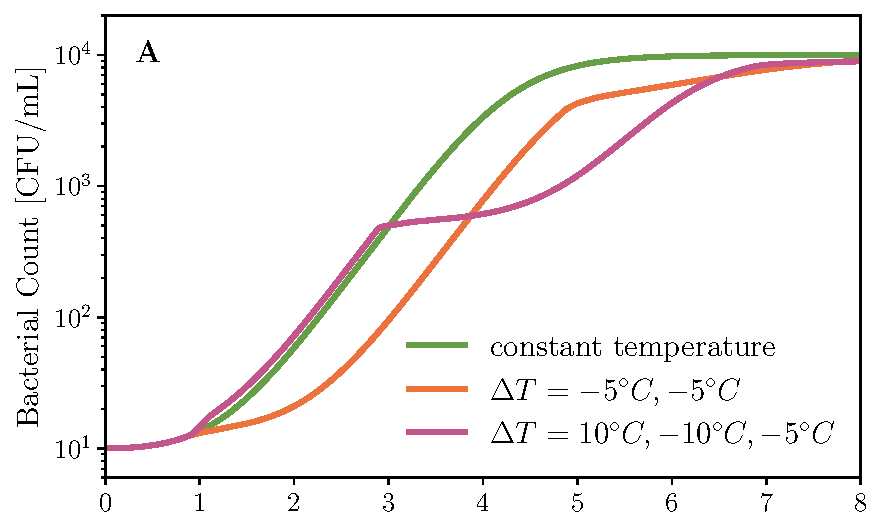
\includegraphics[width=0.9\columnwidth]{Figures-pool_model_3pools_resource_tempshift1.pdf}\\
    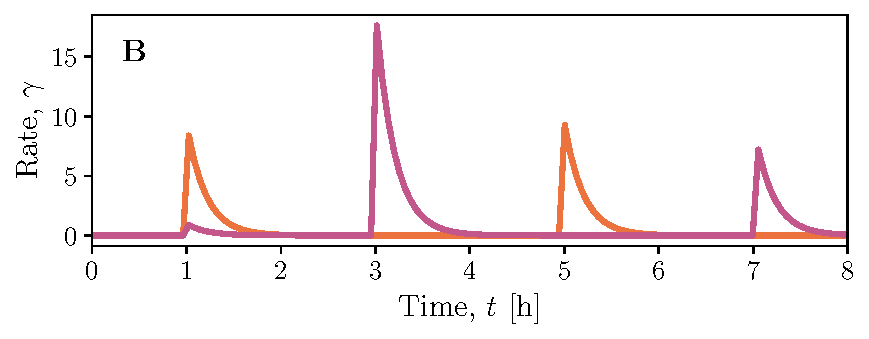
\includegraphics[width=0.9\columnwidth]{Figures-pool_model_3pools_resource_tempshift2.pdf}
    \caption{
        (A) The time dependence of the total bacterial count $\mathcal{N}$ for the model including the transition to dormant state due to temperature stress~(\ref{eq:ode_tempshift_backlag}-\ref{eq:rates_temp_linear}).
        (B) The value of the corresponding flow rate $\gamma$ calculated according to (\ref{eq:gamma_tempshift}) and function~(\ref{eq:f_stress}) with $\alpha=0.05$.
        The curves represent no temperature shift (green), two temperature jumps of $\Delta T = -5~\unit{\degreeCelsius}$ each at times $t=1~\mathrm{h}$ and $t=5~\mathrm{h}$ (orange),
        and the series of different temperature shifts of value $10~\unit{\degreeCelsius}$, $-10~\unit{\degreeCelsius}$, and $-5~\unit{\degreeCelsius}$ at the time points $1~\mathrm{h}$, $3~\mathrm{h}$, and $7~\mathrm{h}$, respectively (rose).
        The parameters associated with dormancy are $\zeta=1~\unit{\hour\per\degreeCelsius}$ and $\delta=5~\mathrm{h}^{-1}$, $\beta=2~\mathrm{h}^{-2}$, $\xi=10^{-3}~\mathrm{h}^{-1}$.
        The growth and lag phase rate linearly depend on the temperature $T$ and are defined as $\mu(T)=0.2 T~\mathrm{h}^{-1}$, $\lambda(T)=10^{-2} T~\mathrm{h}^{-1}$.
        The other model parameters are $\omega'=0.1~\mathrm{h}^{-1}$, $N_t=10^4$, $N_0=10$.
    }
    \label{fig:TempJump}
    \end{center}
\end{figure}
Figure~\ref{fig:TempJump} shows the effect of the temperature shift on the total bacterial count. 
Here, we can observe the asymmetric behavior of the rate $\gamma$ depending on the direction of the temperature change (at $t=1~\mathrm{h}$).
Due to the rapid temperature decrease, the overall growth slows down until dormant bacteria return to the growth pool.
Upon increasing the temperature, the transition into the dormant state is less pronounced ($\alpha=0.05$), such that the effect is negligible; in addition, cell division is stimulated by more favorable conditions~\citep{hamillMicrobialLag2020}.
%
% ================================================================================================
\section{Interaction between species}
As mentioned above, bacteria usually coexist in large interacting communities of multiple species whose growth is largely determined by the survival mechanisms they have developed.
These mechanisms mostly aim to secure a constant availability of nutrients, which leads to competitive strategies or, if it is advantageous, to cooperative ones~\citep{hibbing_bacterial_2010, stubbendieck_bacterial_2016}. Furthermore, we demonstrate that the model can easily be extended to systems with multiple bacterial species in order to describe more complex interspecies relationships.
%
% ------------------------------------------------------------------------------------------------
\subsection{Resource competition}
Competition between bacterial populations can be described in terms of the limiting resource ratio~\citep{tilman_resource_1977, smith_effects_2002,ghoul_ecology_2016}.
To this end, we consider for simplicity only one common limiting resource pool. The simplest pool model for bacterial species $A$ and $B$ encompassing lag phases, growth phases (no back-flow to the lag phase), and a common resource pool is given by:
\begin{align}
    \begin{split}
        \dot{L}_A &= - \lambda_A \tilde{R} L_A\\
        \dot{L}_B &= - \lambda_B \tilde{R} L_B \\
        \dot{G}_A &= \lambda_A \tilde{R} L_A +\mu_A \tilde{R} G_A\\
        \dot{G}_B &= \lambda_B \tilde{R} L_B +\mu_B \tilde{R} G_B\\
        \dot{\tilde{R}} &=-\frac{\mu_A}{N_t} \tilde{R} G_A-\frac{\mu_B}{N_t} \tilde{R} G_B.
    \end{split}
    \label{eq:model_2sp_resource_comp}
\end{align}
We again rescale the resource pool with its total capacity $N_t$ and find
\begin{equation}
    \tilde{R} =1-\frac{L_A+G_A+L_B+G_B}{N_t}.
    \label{eq:Resource}
\end{equation}
Inserting equation~(\ref{eq:Resource}) into system~(\ref{eq:model_2sp_resource_comp}) yields:
\begin{align}
\begin{split}
    \dot{L}_A &= -\lambda_A  L_A + \frac{\lambda_A}{N_t}L_A\mathcal{N}\\
    \dot{L}_B &= -\lambda_B L_B + \frac{\lambda_B}{N_t}L_B\mathcal{N}\\
    \dot{G}_A &=  \lambda_A  L_A + \mu_A G_A - \frac{\lambda_A L_A + \mu_A G_A}{N_t}\mathcal{N}\\
    \dot{G}_B &=  \lambda_B L_B + \mu_B G_B - \frac{\lambda_B L_B + \mu_B G_B}{N_t}\mathcal{N},
    \end{split}
\end{align}
where we used the total bacterial count $\mathcal{N}=(L_A+G_A+L_B+G_B)$.
These equations have the structure of a \ac{glv} model augmented with multiple internal states per species and a resource pool.
As shown in Figure~\ref{fig:2pool_resource_2sp}, even without any direct interaction between species, the bacterial growth was inhibited due to the limitation of the resource. Here species $A$ has a longer lag phase than $B$, but the exponential growth of $A$ is faster than that of $B$.
As a result, species $A$ was able to suppress $B$, by consuming a larger amount of nutrients and reaching a larger bacterial count at steady state.
\begin{figure}[H]
    \begin{center}
    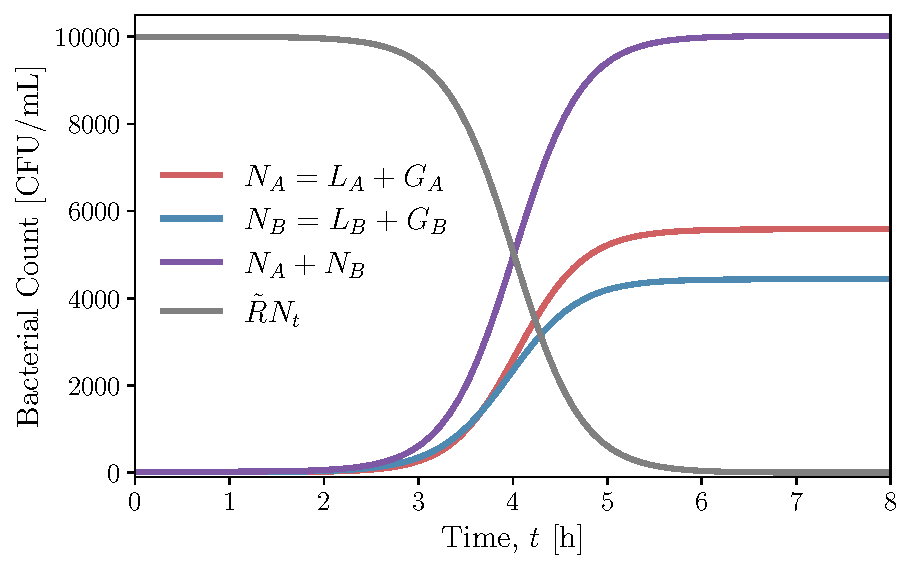
\includegraphics[width=0.9\columnwidth]{Figures-pool_model_2pools_resource_competition.pdf}
    \caption{
        The competition of the two bacterial species due to the common limiting resource calculated using equations~(\ref{eq:model_2sp_resource_comp}).
        The red curve describes the growth of the bacteria $A$ ($N_A = L_A+G_A$) with model parameters $\lambda_A=10^{-2}~\mathrm{h}^{-1}$, $\mu_A=3.0~\mathrm{h}^{-1}$.
        The blue curve describes the growth of the bacteria $B$ ($N_B = L_B+G_B$) with model parameters $\lambda_B=5\cdot 10^{-2}~\mathrm{h}^{-1}$, $\mu_B=2.5~\mathrm{h}^{-1}$.
        The purple line shows the total bacterial count of the system  $\mathcal{N}(t)=N_A+N_B$.
        The gray line denotes the dynamics of the resource pool scaled with its capacity $N_t=10^4$. Initial conditions are $L_A(0)=L_B(0) = 10$, $\tilde{R}(0)=1$.
    }
    \label{fig:2pool_resource_2sp}
    \end{center}
\end{figure}
%
To obtain the standard form of the \ac{glv}, we omit the bacterial states $L_A=L_B=0$:
\begin{align}
    \begin{split}
        \dot{G}_A &= \mu_A G_A\left(1 - \frac{G_A}{N_t}\right) - \frac{\mu_A}{N_t}G_AG_B\\
        \dot{G}_B &= \mu_B G_B\left(1-\frac{G_B}{N_t}\right) -\frac{\mu_B}{N_t}G_AG_B. 
    \label{eq:LV_simple}
    \end{split}
\end{align}
%
Equations (\ref{eq:LV_simple}) can be understood as competitive Lotka-Volterra equations that are widely used in ecological studies and show the principle of competitive exclusion.
This principle states that species competing for the same resource cannot coexist~\citep{wangersky_lotka-volterra_1978}.
Previous studies have shown that \ac{glv} equations with one bacterial state can be successfully applied to predict microbial community dynamics and determine different types of pairwise interspecies interactions~\citep{dedrick_when_2023, stein_ecological_2013, venturelli_deciphering_2018, hoffmann_power_2007}.
In food studies, the \ac{glv} was applied by \citet{mounier_microbial_2008} to study interactions of six bacterial species influenced by yeast omissions in cheese.
\citet{cauchie_modeling_2020} applied the Lotka-Volterra model in their study of the three-species bacterial system in minced pork meat.\\
%
However, in contrast to the classical Lotka-Volterra approach, the introduced pool model allows for far more flexibility in tuning properties of the bacterial interactions within and between species.
For further comparison of the derived model with the matrix formulation of the \ac{glv} we refer the reader to the Appendix~\ref{ssec:supplement1}.
%
%
% ------------------------------------------------------------------------------------------------
\subsection{Interspecies interaction}
Mutual inhibition often results from active competition mechanisms developed by bacteria to compete for a shared resource.
Examples of such mechanisms include the production of antimicrobial compounds, toxins~\citep{wloch-salamon_effect_2008, chao_structured_1981} (section~\ref{section:toxin-production}), or inhibitors~\citep{lenski_coexistence_1986} (section~\ref{section:inhibition}).
On the other hand, some bacteria can produce public goods, the compounds that benefit the growth of other species.
In this way, they can suppress the non-preferred species by helping their competitors~\citep{hibbing_bacterial_2010}.
%
% ................................................................................................
\subsubsection{Amensalism, Toxin production}
\label{section:toxin-production}
One direct form of inhibition is the production of toxins~\citep{cotterBacteriocinsDeveloping2005, rileyBacteriocinsEvolution2002}.
To introduce active competitive mechanisms, we extend our model by having one of the species produce the toxic compounds $\mathcal{T}$ during its growth:
\begin{equation}
    \dot{\mathcal{T}} = \mathcal{F}(\tilde{R},G).
\end{equation}
The function $\mathcal{F}$ denotes the model for the toxin production rate.
One example is the accumulation of bacterial waste that is responsible for the spoilage of food products and suppression of growth of other species.
Consider the system of two species competing for resource $\tilde{R}$ with the production of the toxin $\mathcal{T}$ by species $B$.
We assume that the toxin causes the death of the species $A$ with rate $\omega'$.
Then the full \ac{ode} system is
\begin{align}
    \begin{split}
        \dot{L}_A &= - \lambda_A \tilde{R} L_A\\
        \dot{L}_B &= - \lambda_B \tilde{R} L_B \\
        \dot{G}_A &= \lambda_A \tilde{R} L_A + \mu_A \tilde{R} G_A - \frac{\omega'}{N_t} \mathcal{T}_B G_A\\
        \dot{G}_B &= \lambda_B \tilde{R} L_B + \mu_B \tilde{R} G_B\\
        \dot{\tilde{R}} &= -\frac{\mu_A}{N_t} \tilde{R} G_A-\frac{\mu_B}{N_t} \tilde{R} G_B\\
        \dot{\mathcal{T}}_{B}^{1,2} &= \mathcal{F}^{1,2} (\tilde{R}, G_B),
    \end{split}
    \label{eq:model_2sp_toxin}
\end{align}
%
where we consider two possible models of the toxin production:
\begin{align}
    \mathcal{F}^1(\tilde{R},G_B)&=\kappa G_B\\
    \mathcal{F}^2(\tilde{R},G_B)&=\kappa \tilde{R} G_B
\end{align}
with $\kappa$ as the toxin production rate. The difference in the solutions of the given \acp{ode} between the two toxin production models is presented in Figure~\ref{fig:2pool_2sp_toxin}.
%
%
\begin{figure}[H]
    \begin{center}
    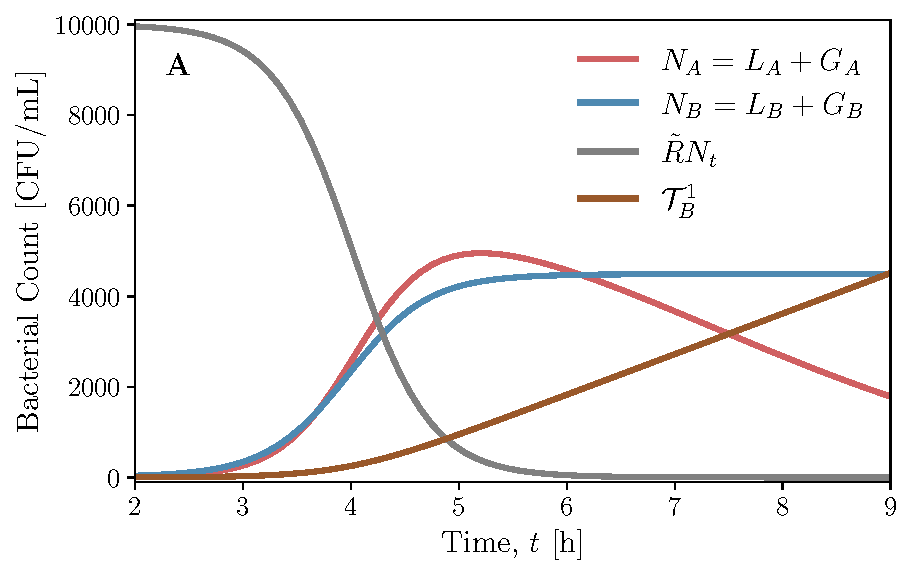
\includegraphics[width=0.9\columnwidth]{Figures-pool_model_2pools_toxin1.pdf}\\
    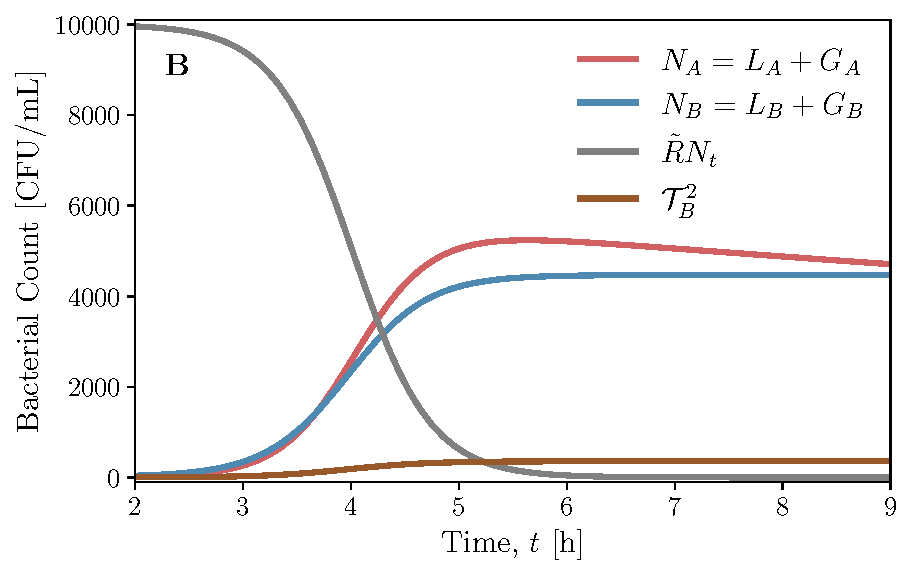
\includegraphics[width=0.9\columnwidth]{Figures-pool_model_2pools_toxin2.pdf} 
    \caption{
        The two-species system with competition for the common nutrient $\tilde{R}$ and production of the toxin $\mathcal{T}_B$ (brown line) calculated using equations~(\ref{eq:model_2sp_toxin}).
        The growing bacteria $B$ produces toxin $\mathcal{T}_B$ (A) constantly $\dot{\mathcal{T}}_B^1 = \mathcal{F}^1 = \kappa G_B$ or (B) only during the growth process $\dot{\mathcal{T}}_B^2 = \mathcal{F}^2 = \kappa \tilde{R} G_B$ 
        with production rate $\kappa=0.2~\mathrm{h}^{-1}$.
        The toxin $\mathcal{T}_B$ causes the cell death of bacteria $A$ with rate constant $\omega' = 1~\mathrm{h}^{-1}$.
        The red curve describes the growth of the bacteria $A$ ($N_A = L_A+G_A$) with model parameters $\lambda_A=10^{-2}~\mathrm{h}^{-1}$, $\mu_A=3.0~\mathrm{h}^{-1}$.
        The blue curve describes the growth of the bacteria $B$ ($N_B = L_B+G_B$) with model parameters $\lambda_B=5\cdot 10^{-2}~\mathrm{h}^{-1}$, $\mu_B=2.5~\mathrm{h}^{-1}$.
        The gray line denotes the dynamics of the resource pool scaled with its capacity $N_t=10^4$. Initial conditions are $L_A(0)=L_B(0) = 10$, $\tilde{R}(0)=1$.
    }
    \label{fig:2pool_2sp_toxin}
    \end{center}
\end{figure}
%
Model $\mathcal{F}^1$ results in toxin concentration $\mathcal{T}_B^1(t)=\kappa\int_{0}^tG_B(t')dt'$.
The production of toxin only depends on the presence of bacteria $G_B$ and is independent of their growth dynamics.
On the other hand, model $\mathcal{F}^2$ assumes that toxin is only produced during bacterial growth and division, and therefore depends on the growth dynamics of $B$.
This leads to a toxin accumulation in the steady state $\mathcal{T}_B^{2s}=\lim_{t\to\infty}\mathcal{T}_B^2(t)=(\kappa/\mu_B)(G_B^s-N_{B0})$; $G_B^s$ denotes the steady state of $G_B$ and $N_{B0}$ the initial concentration of bacteria $B$.
To see this, we note $\dot{\mathcal{T}}_B^2=(\kappa/\mu_B)(\dot{L}_B+\dot{G}_B)$, which yields: $\mathcal{T}_B^2(t)=(\kappa/\mu_B)(L_B(t)+G_B(t)-N_{B0})$ where we used $\mathcal{T}_B^2(0)=G_B(0)=0$, $L_B(0)=N_{B0}$.
%
% ................................................................................................
\subsubsection{Amensalism, Mutual inhibition}
\label{section:inhibition}
Another special case of interspecies competition arises when the toxin produced does not cause the death of the bacteria but rather inhibits their growth.
Such a situation with two bacterial species, a shared resource, and a secreted inhibitor was modeled by \citet{lenski_coexistence_1986}.
The same effect can be modeled by our pool model. We consider a simplified case that reduces the number of variables.
The simplest approach is to assume that the growth rate of species $A$ depends on the abundance of species $B$, and vice versa.
For the sake of simplicity, we ignore the lag pool and describe the growth components via:
\begin{align}
    \dot{G}_A &= \mathcal{B}_A(G_B)G_A\left(1 - \frac{G_A+G_B}{N_t}\right)\\
    \dot{G}_B &= \mathcal{B}_B(G_A) G_B\left(1-\frac{G_A+G_B}{N_t}\right)
\end{align}
The functions $\mathcal{B}_{A/B}$ are a phenomenological choice to capture the inhibiting effects.
It is straightforward to make the mechanism of inhibition more explicit by, e.g., introducing a toxin pool.
One possible choice for $\mathcal{B}$ is:
\begin{equation}
    \mathcal{B}(G) = \frac{\mu}{1+KI(G)}
\end{equation}
where $I$ is the concentration of the inhibiting metabolic byproduct of the bacterial growth.
This leads to
\begin{align}\begin{split}
    \dot{G}_A &= \frac{\mu_A G_A}{1+K_BG_B}\left(1 - \frac{G_A+G_B}{N_t}\right)\\
    \dot{G}_B &= \frac{\mu_B G_B}{1+K_AG_A}\left(1-\frac{G_A+G_B}{N_t}\right).
\end{split}\end{align}

One can distinguish two limiting cases: {\it i}) $K_{A/B}\ll N_t$ and {\it ii}) $K_{A/B}\gg N_t$.
In the first case, the inhibition is of minor importance and could be ignored, while in the latter case one can simplify the equations, given $G_A$ and $G_B$ are non-zero:
\begin{align}\begin{split}
    \dot{\tilde{G}}_A &=\tilde{\mu}_A\frac{\tilde{G}_A}{\tilde{G}_B}\left(1 - \tilde{G}_A-\tilde{G}_B\right)\\
    \dot{\tilde{G}}_B &= \tilde{\mu}_B\frac{\tilde{G}_B}{\tilde{G}_A}\left(1 - \tilde{G}_A-\tilde{G}_B\right).
\end{split}\end{align}
We introduced the rescaled growth rates $\tilde{\mu}_A=\mu_A/(N_tK_B)$ and $\tilde{\mu}_B=\mu_B/(N_tK_A)$ and rescaled $\tilde{G}_A=G_A/N_t$ and $\tilde{G}_B=G_B/N_t$.
Note that $[\tilde{\mu}_{A/B}]=\mathrm{h}^{-1}$.
We further rescale time with $\tilde{\mu}_A$ and define the dimensionless parameter
\begin{equation}
    \psi = \tilde{\mu}_B/\tilde{\mu}_A = \frac{K_B\mu_B}{K_A\mu_A},
\end{equation}
which results in
\begin{align}
    \begin{split}
        \dot{\tilde{G}}_A &=\frac{\tilde{G}_A}{\tilde{G}_B}\left(1 - \tilde{G}_A-\tilde{G}_B\right)\\
        \dot{\tilde{G}}_B &=\psi\frac{\tilde{G}_B}{\tilde{G}_A}\left(1-\tilde{G}_A-\tilde{G}_B\right). 
    \end{split}
\label{eq:2sp_1pool_inhibit_unitless}
\end{align}
We can separate three cases:
\begin{align}
    \psi&=1:\quad\text{A and B are equivalent}\\
    \psi&>1:\quad\text{B grows faster/inhibits A}\\
    \psi&<1:\quad\text{A grows faster/inhibits B},
\end{align}
which are displayed in Figure~\ref{fig:1pool_2sp_inhibit}.
The advantage of this system is its simplicity, allowing us to describe the effect of mutual inhibition between two bacterial species with only a single parameter.
%
\begin{figure}[H]
    \begin{center}
    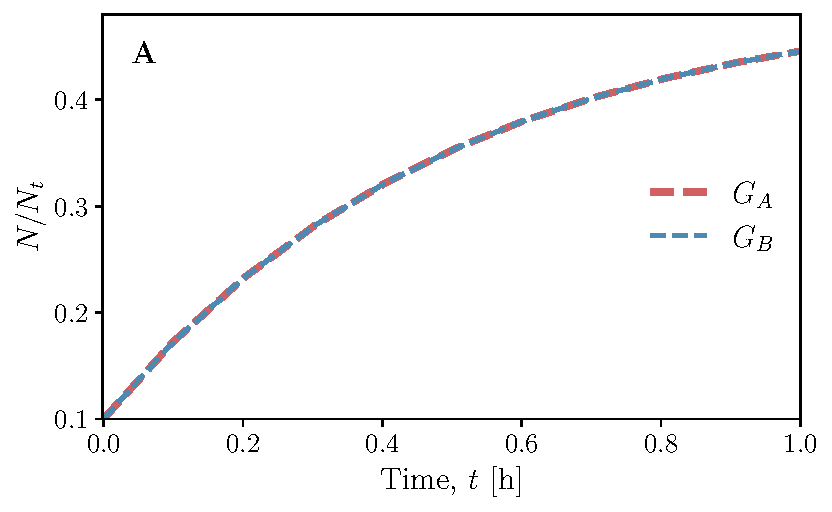
\includegraphics[width=0.32\textwidth]{Figures-pool_model_1pool_inhib1.pdf}
    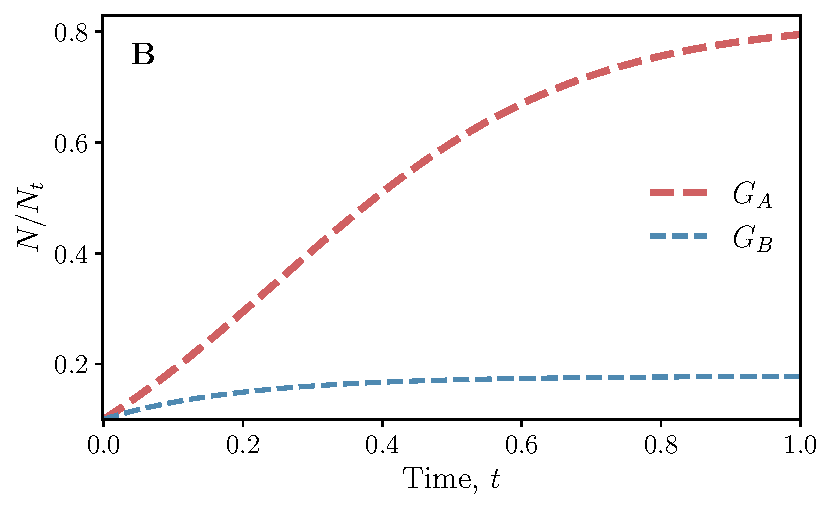
\includegraphics[width=0.32\textwidth]{Figures-pool_model_1pool_inhib2.pdf}
    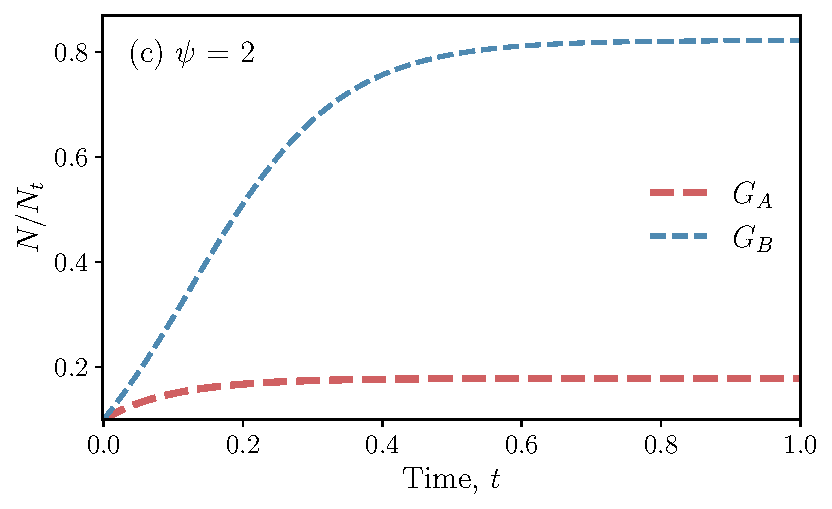
\includegraphics[width=0.32\textwidth]{Figures-pool_model_1pool_inhib3.pdf}\\
    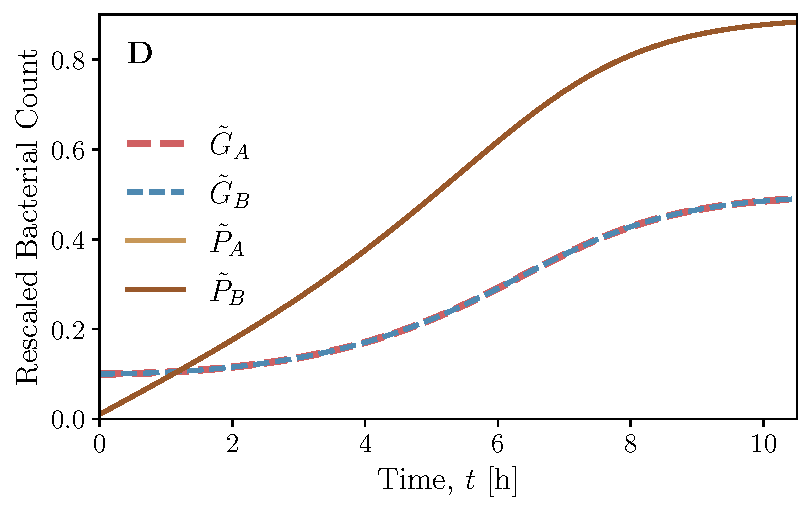
\includegraphics[width=0.32\textwidth]{Figures-pool_model_2sp_1pool_coop1.pdf}
    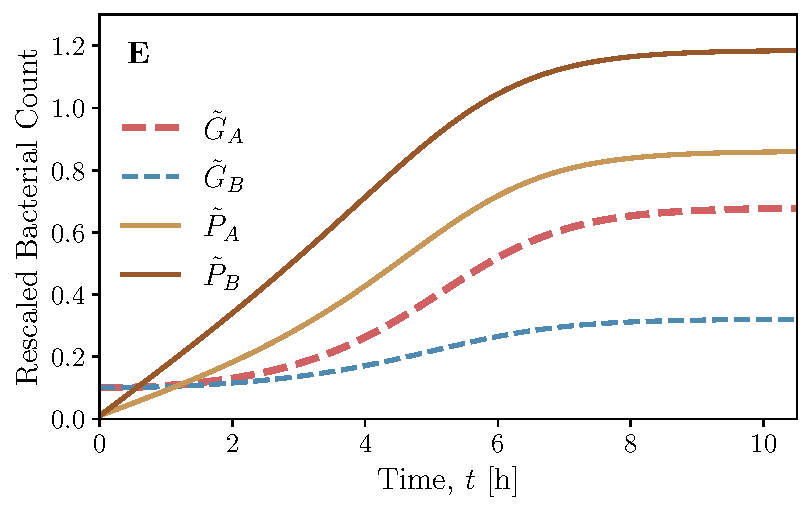
\includegraphics[width=0.32\textwidth]{Figures-pool_model_2sp_1pool_coop2.pdf}
    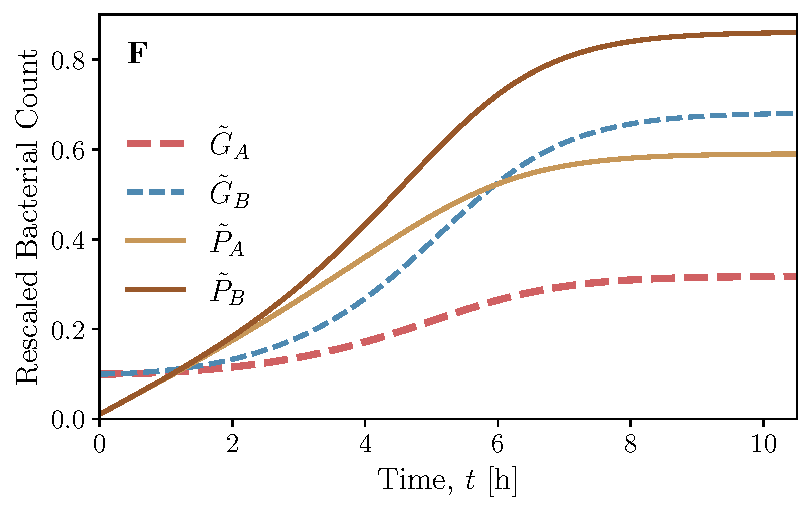
\includegraphics[width=0.32\textwidth]{Figures-pool_model_2sp_1pool_coop3.pdf}
    \caption{
        (A) - (C) The two-species system mutually inhibiting each other, described by equations~(\ref{eq:2sp_1pool_inhibit_unitless}).
        Here the red lines describe the evolution of species $A$ and the blue lines correspond to species $B$.
        The relation between the inhibition strength of species $B$ and $A$ is defined by the control parameter value (A) $\psi$ = 1, (B) $\psi$ = 0.5, or (C) $\psi$ = 2.\\
        (D) - (F) The two-species system where each of the species releases public goods $P$, described by equations~(\ref{eq:1pool_2sp_cooper}) and calculated for different parameters:
        (D) $\chi=1, \phi=1$, (E) $\chi=1, \phi=2$, and (F) $\chi=2, \phi=1$.
        Here the red lines describe the evolution of species $A$ and the blue lines correspond to species $B$.
        The light brown curve corresponds to the public good released by species $A$ ($\tilde{P}_A$) and the brown curve shows the public goods produced by species $B$ ($\tilde{P}_B$). Initial conditions are
        $\tilde{G}_A(0)=\tilde{G} _B(0)=0.1$ and $\tilde{P}_A(0)=\tilde{P}_B(0)=0.01$. Note the different time scales in panels (A)–(C) and (D)–(F).
    }
    \label{fig:1pool_2sp_inhibit}
    \end{center}
\end{figure}
%
% ------------------------------------------------------------------------------------------------
\subsection{Mutualism, Interspecies cooperation}
On the other hand, one can also observe some cooperative behaviors between species in cases where cooperation facilitates competition with others.
This phenomenon occurs due to complementary metabolic pathways, i.e., the production of so-called public goods that benefit the growth of other species. It is most often observed between closely related species or clonal populations, a process called kin selection~\citep{west_social_2007}.
Furthermore, neighbors can also benefit from a behavior that does not require any action at the gene expression level, the so-called 'social cheaters'~\citep{rainey_evolution_2003}.
This mutual activation benefits all participating species and can be easily included in our mathematical framework.
For the sake of clarity, we again omit the lag pool and write:
\begin{align}
	\begin{split}
    \dot{G}_A &= \mathcal{B}_A(P_B,\tilde{R})G_A\\
    \dot{G}_B &= \mathcal{B}_B(P_A,\tilde{R})G_B\\
    \dot{\tilde{R}} &=-\mathcal{B}_A(P_B,\tilde{R})G_A-\mathcal{B}_B(P_A,\tilde{R})G_B\\
    \dot{P}_A &= \mathcal{F}_A(\tilde{R},G_A)\\
    \dot{P}_B &= \mathcal{F}_B(\tilde{R},G_B),
    \end{split}
\end{align}
where $P_A$ and $P_B$ denote the substance produced by species A and B, respectively.
The functions $\mathcal{B}_A(P_B,\tilde{R})$ and $\mathcal{B}_B(P_A,\tilde{R})$ capture the resource-dependent growth.
We set $\mathcal{B}_A(P_B,\tilde{R})=(\mu_A/N_t) P_B\tilde{R}$, $\mathcal{B}_B(P_A,\tilde{R})=(\mu_B/N_t) P_A \tilde{R}$, $\mathcal{F}_A(\tilde{R},G_A)=\kappa_A \tilde{R}G_A$, $\mathcal{F}_B(\tilde{R},G_B)=\kappa_B \tilde{R}G_B$.\\

Exploiting $N_t \tilde{R}(t)+G_A(t)+G_B(t)=N_t$ (note, $[\tilde{R}]=1$), rescaling $G_A$, $G_B$, and $P_B$ with $N_t$, $P_A$ with $\kappa_A/\mu_A$, time with $\mu_A N_t$, defining $\chi=\kappa_A\mu_B/(\mu_A^2N_t)$, and $\phi=\kappa_B/(\mu_A N_t)$ results in:
\begin{align}
    \begin{split}
        \dot{\tilde{G}}_A &= \tilde{P}_B \tilde{G}_A\left(1 - \tilde{G}_A-\tilde{G}_B\right)\\
        \dot{\tilde{G}}_B &= \chi \tilde{P}_A \tilde{G}_B\left(1 - \tilde{G}_A-\tilde{G}_B\right)\\
        \dot{\tilde{P}}_A &= \tilde{G}_A\left(1 - \tilde{G}_A-\tilde{G}_B\right)\\
        \dot{\tilde{P}}_B &=\phi \tilde{G}_B\left(1 - \tilde{G}_A-\tilde{G}_B\right).
    \end{split}
    \label{eq:1pool_2sp_cooper}
\end{align}
%
The solution of the system~(\ref{eq:1pool_2sp_cooper}) is presented in Figure~\ref{fig:1pool_2sp_inhibit}.
Here we can see that if $\chi=1$ and $\phi=1$, the production rate of the public goods of both species is identical to the growth rate of bacteria (see Figure~\ref{fig:1pool_2sp_inhibit}D).
Increasing the production rate of the public good (see Figure~\ref{fig:1pool_2sp_inhibit}E) leads to an increase in the growth of species $A$ that profits from the presence of $B$.
On the other hand, choosing $\chi=2$ (see Figure~\ref{fig:1pool_2sp_inhibit}F), we increase the profit that species $B$ has from public goods $\tilde{P}_A$.
This indirectly leads to a larger amount of $\tilde{P}_B$ produced by species $B$.
% ================================================================================================
\section{Spatial effects}
The pool model does not account for the spatial bacterial distribution. Assuming that the bacterial system is uniformly distributed (sometimes also called 'well-stirred'),
we expect the \ac{ode} description to be valid. However, in reality, spatial effects can play a significant role in population survival, forcing some
species to develop competitive mechanisms such as cell adhesion to surfaces in areas rich in
nutrients~\citep{htuson_bacteriasurface_2013}.
Another mechanism is the motility of bacteria, e.g., flagellated \textit{E. coli} or
\textit{B. subtilis}, which are capable of chemotactic motion driven by oxygen
concentrations~\citep{decoene_microscopic_2011}. Bacterial social interactions such as the release of toxins or public goods can also significantly affect the spatial structure of the community~\citep{blanchard_bacterial_2015}. These effects can only be treated within a spatial framework capable of capturing them.\\

Compared to other modeling techniques such as \acp{pde}, \acp{abm}~\citep{nagarajan_agent-based_2022-1} force researchers to think in
terms of cellular processes, thus bridging the gap from a collective (bulk) model to an individual-based (single-cell) description. Our goal is to provide an \ac{abm} that can be used to derive the given \ac{ode} model as a coarse-grained approximation. In this way, we can show that the bulk-based \ac{ode} model is directly related to the mechanistic
single-cell behavior of the bacteria. To this end, we consider a system consisting of two bacterial species that can each be described by the two internal states: lag and growth phase.

Both of these species grow using the same resource pool $\tilde{R}$ but with different growth constants
$\mu_{A/B}$ and different lag phase transition rates $\lambda_{A/B}$.
Moreover, species $A$ is able to release a certain antimicrobial component $I$ that shows an
inhibitory effect on species $B$ (amensalism). The \acp{ode} system of the bacterial population can be written as:
%
\begin{align}
    \begin{split}
        \dot{L}_A &= -\lambda_A \tilde{R} L_A\\
        \dot{G}_A &= \lambda_A \tilde{R} L_A + \mu_A \tilde{R} G_A\\
        \dot{L}_B &= -\lambda_B \tilde{R} L_B\\
        \dot{G}_B &= \lambda_B \tilde{R} L_B + \frac{\mu_B}{1 + K_I I} \tilde{R} G_B.
    \end{split}
    \label{eq:spatial_limit_F}
\end{align}
%
Moreover, the microenvironment of our system contains both the resource and inhibitor molecules
\begin{align}
    \begin{split}
        \dot{\tilde{R}} &= -\frac{\mu_A}{N_t} \tilde{R} G_A-\frac{\mu_B}{(1 + K_I I) N_t} \tilde{R} G_B \\
        \dot{I} &= \kappa G_A.
    \end{split}
    \label{eq:spatial_limit_H}
\end{align}
%
% ------------------------------------------------------------------------------------------------
\subsection{Constructing an agent-based pool model}
The following sections will demonstrate how a given \ac{ode} system can be translated into a custom-built \ac{abm} that requires only a few additional parameters.
This procedure is a blueprint that can be followed to construct \acp{abm} for similar \ac{ode}-based systems.\\

To construct our \ac{abm}, we use the modeling framework \texttt{cellular\_raza}~\citep{Pleyer2025} that allows us to define our bacterial agents from a clean slate.
With this flexibility, researchers are able to construct minimal models using only as many parameters as are necessary. This ability to precisely define and control the exact behavior of the cell-agents enables the developments described below.
%
\subsubsection{Cellular reactions}
To construct an \ac{abm} that resembles the given \ac{ode} system of equations~\eqref{eq:spatial_limit_F} and \eqref{eq:spatial_limit_H}, we consider multiple cellular reactions.
We denote quantities of cellular species $A,B$ with the subscript $c_{A/B}$, respectively. Cells go from the lag phase $L$ to the growth-phase with a given transition probability, modeled as a Markovian process (no memory).  The nutrient concentration $R(x)$ in the microenvironment is potentially spatially inhomogeneous and nutrients diffuse freely with diffusion constant $D_R$. $R(x)$ denotes the non-rescaled resource pool with $[R]=V^{-1}$ in contrast to the rescaled homogeneous pool $\tilde{R}$ in \eqref{eq:spatial_limit_F} and \eqref{eq:spatial_limit_H}. 
Cells take up extracellular resources $R$ and convert them into biomass, which is measured in terms of cellular volume.
Cells of type $A$ release a diffusible molecule into the microenvironment with concentration $I$ and diffusion constant $D_I$, which inhibits the growth of the cells of type $B$.
When combining all of the listed effects and considering multiple cells of the two species $A/B$, we obtain the system:
\begin{alignat}{5}
	\text{Prob}(L\to G) &= \lambda \frac{R(x)}{N_t}\Delta t\\
    \dot{V}_{c_A} &= u_A \sigma R(x_{c_A})V_{c_A}
    \label{eq:spatial-full-system-simplified-begin}\\
    \dot{V}_{c_B} &= \frac{u_B}{1+K_I I(x_{c_B})} \sigma R(x_{c_B}) V_{c_B}\\
    \dot{R}(x) &= -u_A \sum\limits_{c_A}V_{c_A} R(x) \delta(x-x_{c_A})\\
        &\quad- u_B \sum\limits_{c_B}V_{c_B}\frac{R(x) }{1+ K_I I(x)}\delta(x-x_{c_B})\nonumber\\
    \dot{I}(x) &=b\sum\limits_{c_A} V_{c_A}\delta(x-x_{c_A}) + D_I\Delta I(x).
    \label{eq:spatial-full-system-simplified-end}
\end{alignat}
For the diffusion, we require Neumann (zero-flux) boundary conditions.
Note that the sums $\sum_{c_{A/B}}$ range over all cells that are in the growth phase at a given time point. This means explicitly that the number of summands varies in time and is part of the overall dynamics.

\subsubsection{Physical mechanics \& interactions}
We model cells as spherical objects in 2D space. They can be represented by their position $x_c$ and radius $r_c$, which is related to their (2D) volume $V_c = \pi r_c^2$.
As the coupled reactions from equations~\eqref{eq:spatial-full-system-simplified-begin} change $V_c$, we also automatically adapt the cell radius accordingly.
The dynamics are described by Newton's law of motion with viscous damping:
\begin{equation}
    m \ddot{\mathbf{x}} = -\eta\dot{\mathbf{x}} + \mathbf{F}.
\end{equation}
Cells interact via a point-like interaction potential. We can calculate the interaction strength via:
\begin{alignat}{3}
    \mathbf{z} &= \mathbf{x}_1 - \mathbf{x}_2 \hspace{2em}&& r = ||\mathbf{z}||\\
    \rho &= \frac{r}{r_1+r_2} && q=0.2\\
    \mathbf{F} &= \epsilon \frac{1+q}{q+\rho} \theta(1 - \rho) \frac{\mathbf{z}}{r}.
\end{alignat}
The distance between cells is given by $r$; the radii of the cells are $r_1$ and $r_2$, respectively. The parameter $q$ determines the slope of $||\mathbf{F}||$ at $\rho=1$; the larger $q$ is, the shallower the slope. $\epsilon$ denotes the strength of the force at $\rho=1$. 
We ignore any attractive force between the cells and consider only a repulsive interaction potential~\citep{Garrett2008}.
These mechanisms will result in the overall expansion of the colony as individual cells push each other further apart.

\subsubsection{Cell cycle}
Typically, the cycle of a cell consists of multiple phases~\citep{Cooper2000_fn}. Since our goal is to include only the necessary details of the underlying biological problem, we drastically simplify the description of the cell cycle. Cell growth is already being described by the system of coupled \acp{ode} given in equations~\eqref{eq:spatial-full-system-simplified-begin}-\eqref{eq:spatial-full-system-simplified-end}.
Thus, we introduce an additional rule that performs the division process when a certain volume threshold is reached.
The volume of the cell is divided equally between the new and old cells, and both are assigned new random positions close to each other such that their radii touch without overlap (see Figure ~\ref{fig:cell_division}).
\begin{figure}[H]
    \begin{center}
    \begin{tikzonimage}[width=0.49\textwidth]
        {Figures-snapshot-2-cells-before-division.png}%
        \node at (0.01, 0.99)[anchor=north west]{\textbf{A}};
    \end{tikzonimage}%
    \hspace{0.01\columnwidth}%
    \begin{tikzonimage}[width=0.49\textwidth]
        {Figures-snapshot-2-cells-after-division.png}
        \node at (0.01, 0.99)[anchor=north west]{\textbf{B}};
    \end{tikzonimage}
    \caption{
        (A) A cell right before and (B) after a division event.
        The volume is equally distributed between the two cells and the new positions are picked
        randomly but at opposing sides on a circle around the original center of the single cell.
    }
     \label{fig:cell_division}
    \end{center}
\end{figure}
%
%
% ------------------------------------------------------------------------------------------------
\subsection{Comparing \acs{abm} and \acs{ode} models}
\label{subsec:comparigon-abm-and-ode}
The \ac{ode} model can only approximate the \ac{abm} model and becomes asymptotically correct in the limit of fast diffusion and high cell density. The \ac{abm} model is more closely linked to the biology of cells because it incorporates more biological aspects.
By comparing the \ac{ode} model derived from the \ac{abm} with the \ac{ode} equations~\eqref{eq:spatial_limit_F} and \eqref{eq:spatial_limit_H} we find the following relation between the parameters (see Appendix~\ref{sec:supplement-abm-derivation}):
\begin{align}
    \begin{split}
        G_{A/B} &= \frac{1}{\sigma V_D}V_{A/B}\\
        \frac{\mu_{A/B}}{N_t} &= u_{A/B}\sigma\\
        \kappa &= \sigma b. 
    \end{split}
    \label{eq:ode-abm-mappings}
\end{align}
We can use these mappings to numerically compare both approaches. Table~\ref{tab:spatial_limit_init} shows an example comparison of parameters of the \ac{ode} and \ac{abm}. Figure~\ref{fig:spatial-snapshots} shows snapshots of a numerical simulation of the described system. The bacteria are initially ordered on a grid to achieve a more homogeneous initial distribution.
%
\begin{figure}[H]
    \begin{tikzonimage}[width=0.49\textwidth]
        {Figures-abm-homogenous-images-snapshot_00024000.pdf}
        \node at (0.01, 0.99)[anchor=north west]{\textbf{A}};
    \end{tikzonimage}%
    \hspace{0.01\columnwidth}%
    \begin{tikzonimage}[width=0.49\textwidth]
        {Figures-abm-homogenous-images-snapshot_00048000.pdf}
        \node at (0.01, 0.99)[anchor=north west]{\textbf{B}};
    \end{tikzonimage}\\
    \begin{tikzonimage}[width=0.49\textwidth]
        {Figures-abm-homogenous-images-snapshot_00072000.pdf}
        \node at (0.01, 0.99)[anchor=north west, white]{\textbf{C}};
    \end{tikzonimage}%
    \hspace{0.01\columnwidth}%
    \begin{tikzonimage}[width=0.49\textwidth]
        {Figures-abm-homogenous-images-snapshot_00096000.pdf}
        \node at (0.01, 0.99)[anchor=north west, white]{\textbf{D}};
    \end{tikzonimage}%
    \caption{
        \ac{abm} simulation snapshots at $\SI{100}{\minute}$, $\SI{200}{\minute}$, $\SI{300}{\minute}$, and $\SI{400}{\minute}$
        using the parameters given in Table~\ref{tab:spatial_limit_init}. Species $A$ is colored in red while species $B$ is colored in blue. The background shows the resource concentration $R$.
        Darker colors indicate lower nutrient concentration.
    }
    \label{fig:spatial-snapshots}
\end{figure}
%
%
Figure~\ref{fig:spatial-growth-curve} shows results for various configurations of the \ac{abm}, differing only in their initial spatial configuration and diffusivity.
We see that in the highly-diffusive homogeneous case of subfigure (A), the pool model is a good fit for the \ac{abm} model.
This suggests that the ODE model remains suitable for aqueous environments, where homogeneity is more likely.
Heterogeneity and slower diffusion cause larger differences between the two models as can be seen in subfigures (B) and (C).
The combination of the two effects shows the largest difference between model outputs.
In subfigure (C), due to the heterogeneous cell distribution (see Figure~\ref{fig:supplement-spatial-initial-config-cells}), overall inhibition of species $B$ is significantly reduced.
Subfigure (D) shows how a randomized homogeneous initial distribution can lead to even more pronounced effects of inhibition.
In contrast to the other results, here the final values of species $A$ and $B$ have larger or smaller counts, respectively. This illustrates that spatial effects can shift the final results of growth curves toward both directions, leading to an overall increase/decrease of one species. We furthermore note that the total bacterial volume of the \ac{abm} is always less than or equal to that of the \ac{ode} model. This is expected, since processes such as diffusion and cells growing outward introduce an additional time component that is simply assumed to be instantaneous in the \ac{ode} model.
From studies on the branching patterns of bacterial colonies~\citep{Kawasaki1997,Matsushita1998}, we know that the diffusivity of
nutrients is of the order of the spatial extension rate of the bacterial colony. The chosen diffusion constants $D_I=D_R\in\{2, 20\}~\unit{\micro\metre\squared\per\second}$ are representative of fast- and slow-diffusing systems, respectively.
\begin{figure}[H]
    \centering
    \begin{tikzonimage}[width=0.49\textwidth]
        {Figures-abm-homogenous-abm_ode_comparison.pdf}
        \node at (0, 1)[anchor=north west]{\textbf{A}};
    \end{tikzonimage}%
    \begin{tikzonimage}[width=0.49\textwidth]
        {Figures-abm-homogenous-low-diffusion-abm_ode_comparison.pdf}
        \node at (0, 1)[anchor=north west]{\textbf{B}};
    \end{tikzonimage}\\
    \begin{tikzonimage}[width=0.49\textwidth]
        {Figures-abm-inhomogenous-abm_ode_comparison.pdf}
        \node at (0, 1)[anchor=north west]{\textbf{C}};
    \end{tikzonimage}%
    \begin{tikzonimage}[width=0.49\textwidth]
        {Figures-abm-random-abm_ode_comparison.pdf}
        \node at (0, 1)[anchor=north west]{\textbf{D}};
    \end{tikzonimage}
    \caption{
        (A-D) Comparison of the \ac{ode} (solid lines) and \ac{abm} (dashed lines) model for different configurations.
        (A) Homogeneous, fast diffusion, 
        (B) Homogeneous, slow diffusion, 
        (C) Heterogeneous, fast diffusion, 
        (D) Random, fast diffusion.
        The diffusion constants are chosen such that $D_R=D_I\in\{2, 20\}~\unit{\micro\metre\squared\per\second}$.
        Snapshots of the spatial configurations of cells are shown in Figure~\ref{fig:supplement-spatial-initial-config-cells}.
    }
    \label{fig:spatial-growth-curve}
\end{figure}
These results show how variations in properties that cannot be described by \ac{ode} models can lead to large deviations in the growth curves of the species.
%
% ================================================================================================
\section{Discussion}
%
The pool model introduced in this work provides a flexible, mechanistic framework
for describing bacterial growth and interspecies interactions at the population level.
By partitioning the bacterial population into discrete metabolic states and defining
biologically motivated transitions between them, a wide range of phenomena can be
captured with a minimal and interpretable set of parameters.

The three-pool model with a limiting resource yields growth curves qualitatively
comparable to established primary models in predictive microbiology, including the
Baranyi-Roberts model~\citep{baranyi_dynamic_1994} and the McKellar
two-compartment model~\citep{McKellar1997}, while offering a clearer mechanistic interpretation of each parameter.

The dormancy extension illustrates a key strength of the pool model: new biological
states can be incorporated systematically without restructuring the existing equations.
The proposed Maxwell-type relation for the stress rate reproduces the
experimentally observed asymmetric response of bacteria to temperature increases and
decreases~\citep{swinnen_predictive_2004, hamillMicrobialLag2020}.

The multi-species extensions show that the pool model subsumes several established
model classes. Omitting the lag pool causes the resource competition equations to reduce exactly to the generalized Lotka-Volterra equations~\eqref{eq:LV_simple}. This establishes a direct mathematical connection between the pool framework and one of the most widely used formalisms in microbial ecology~\citep{wangersky_lotka-volterra_1978,
stein_ecological_2013, venturelli_deciphering_2018}.
The two toxin production models highlight how different biological assumptions lead to
qualitatively distinct dynamics. The mutual inhibition model further demonstrates that complex competitive exclusion
dynamics can be captured with a single dimensionless parameter, greatly
reducing model complexity without sacrificing mechanistic interpretability. Furthermore, the mutualism model shows that cooperative interspecies dynamics, 
such as the cross-feeding of public goods observed in mixed-culture fermentations, can be described with only two dimensionless parameters, which quantify the asymmetry of the mutualistic benefit between the two species.

The \ac{abm} analysis reveals the conditions under which the \ac{ode} approximation
is valid. In the highly-diffusive, homogeneous case (Figure~\ref{fig:spatial-growth-curve}A),
\ac{ode} and \ac{abm} agree closely, supporting the use of \ac{ode} models in aqueous
environments with rapid nutrient transport.
Slower diffusion or heterogeneous initial cell distributions introduce systematic
deviations: in particular, a heterogeneous cell distribution
(Figure~\ref{fig:spatial-growth-curve}C) significantly reduces the inhibition of
species $B$ by the antimicrobial compound of species $A$, since spatial separation
limits exposure.
Conversely, a random initial distribution (Figure~\ref{fig:spatial-growth-curve}D) can
amplify inhibition effects relative to the \ac{ode} prediction.
In all configurations, the total bacterial volume of the \ac{abm} is less than or equal to
that of the \ac{ode} model, as diffusion and outward colony expansion introduce
delays that the \ac{ode} formulation treats as instantaneous.

Several limitations of the current framework should be noted.
The \ac{ode} model assumes a well-mixed population, which may not hold in biofilms or
spatially confined food matrices.
The stress-rate parameters of the dormancy model are
phenomenological and may be difficult to determine from standard plate-count
experiments without dedicated temperature-shift protocols.
Finally, stochastic effects -- relevant at low cell numbers, for example during early
colonization of a food surface -- are not captured by the \ac{ode} formulation.
%
% ------------------------------------------------------------------------------------------------
\section{Conclusion}
%
We introduced the pool model as a unifying, mechanistic framework for modeling
bacterial consortia in food science.
The framework describes bacterial populations in terms of discrete metabolic states
and transitions between them, providing a systematic route from first-principles
assumptions about single-cell behavior to population-level \acp{ode}.
Applied to one- and two-species systems, it reproduces the growth dynamics of
established primary models while remaining more interpretable, and it naturally
generalizes the \ac{glv} equations as a special case.
By deriving the pool model equations from an explicit \ac{abm}, we have shown that the
framework directly reflects individual cell-level biological processes, bridging the
gap between mechanistic single-cell descriptions and coarse-grained population models.
Going forward, the framework can be extended to additional internal states and
environmental drivers -- such as pH, water activity, or quorum sensing -- by including
new pools and secondary models for the transition rates, providing a flexible starting
point for predictive microbiology in food safety applications.

\newpage
\section*{Data availability \& reproducibility}
The data and simulation code that are presented in this study are publicly available at
\url{https://github.com/polinagaindrik/pool_model_paper}.

\section*{Declaration of competing interest}
The authors declare no conflict of interest.

\section*{Acknowledgements}
P.G. and C.F. received funding from the FutureLab program (grant 281K126A20) of the Federal Ministry of Food and Agriculture (Bundesministerium für Ernährung und Landwirtschaft, BMEL). J.P. and C.F. received funding from a FET-Open research and innovation actions grant under the European Union's Horizon 2020 program (CyGenTiG; grant agreement 801041).

\section*{Author Contributions}
\begin{tabularx}{\textwidth}{l @{\hspace{0.5cm}} l}
    \textbf{Conceptualization}              	& Christian Fleck, Matthias Brunner\\
    \textbf{Analysis - \acs{ode} Models}	& Polina Gaindrik, Christian Fleck\\
    \textbf{Analysis - Spatial effects}		& Jonas Pleyer, Christian Fleck\\
    \textbf{Writing}                        		& Christian Fleck, Polina Gaindrik, Jonas Pleyer, Fernando Pérez Rodríguez, Matthias Brunner\\
    \textbf{Supervision}                  		& Christian Fleck\\
    \textbf{Funding acquisition} 	    		& Christian Fleck, Matthias Brunner
\end{tabularx}

% \printbibliography
\bibliography{references.bib}

% ================================================================================================
\newpage

\newcounter{suppsection}
\newcounter{supptable}
\newcounter{suppfigure}
% \newcounter{suppequation}

\renewcommand{\thesection}{S\arabic{suppsection}}
\renewcommand{\thetable}{S\arabic{supptable}}%
\renewcommand{\thefigure}{S\arabic{suppfigure}}%
% \renewcommand{\theequation}{S\arabic{suppequation}}%

\let\oldsection\section
\let\oldtable\table
\let\oldfigure\figure
\makeatletter
\renewcommand{\section}{\@ifstar{\oldsection*}{\stepcounter{suppsection}\oldsection}}
\renewcommand{\table}{\@ifstar{\oldtable*}{\stepcounter{supptable}\oldtable}}
\renewcommand{\figure}{\@ifstar{\oldfigure*}{\stepcounter{suppfigure}\oldfigure}}
\makeatother

\addcontentsline{toc}{Section}{Supplementary Material}% Add section to ToC

% ================================================================================================
\section{General mathematical formalism}
\label{ssec:supplement1}
Consider the system consisting of $N$ species in $M$ different states.
In the general representation, all systems discussed in the main part can be described by the Ordinary Differential Equations (\acp{ode}) using a non-linear function $\mbF$:
\begin{equation}
   \dot{\mbx} = \mbF(\mbx, \mbm, \mbp, \mbu),
\label{eq:model_ODE_x}
\end{equation}
where  $\mbx \in \mathbb{R}^{N}  \otimes \mathbb{R}^{M}$ is a vector describing bacterial count.
In matrix form it can be written as:
\begin{equation}
    \mbx = \begin{pmatrix}
        x^1_1  & \dots & x^1_N  \\
        \vdots &       & \vdots \\
        x^M_1  & \dots & x^M_N  \\
            \end{pmatrix},
    \label{eq:model_bact}
\end{equation}
with $x_{j}^{i}$ describing the bacterial counts for species $i$ in state $j$.
$\mbu$ is the vector of various inputs into the model, e.g., temperature, pressure, etc.
The vector $\mbm \in \mathbb{R}^{K}$ includes all variables corresponding to the microenvironment of the system that can be, e.g., concentrations of inhibitors or activators:
\begin{equation}
    \dot{\mbm} = \mbH (\mbx, \mbm, \mbp, \mbu).
    \label{eq:model_microenv}
\end{equation}
The function $\mbH$ is in the general case also non-linear.\\
%
The advantage of this formulation is its generality. Depending on the knowledge about the system as well as the needed level of accuracy, one can control the complexity of the model by defining an appropriate number $M$ of internal states.\\
%
To obtain the bacterial count for one species $i$, we simply need to sum the tensor $\mbx$ over all possible states:
\begin{equation}
    N_i = \sum_k \mbx_i^k.
\label{eq:N_pro_species}
\end{equation}
The total bacterial count of all species of our system is given by:
\begin{equation}
    \mathcal{N} = \sum_i \sum_k \mbx_i^k.
\label{eq:N_total}
\end{equation}
%
%
%
Using such matrix representation of the bacterial system, we can rewrite, for example, the three-pool model with limited resources described by equation~(\ref{eq:ode_3pool_resource}) in a more compact form. The concentrations of the pools are then the components of our variable vector $\mbx (t) = (L(t), G(t), D(t))^T$.
%
\begin{align}
    \dot \mbx  &= \mbF(\mbx, \mbm, \mbp, \mbu) = \begin{pmatrix}
        -(\omega + \lambda) & 0               & 0      \\
        \lambda          & \mu \tilde{R} - \omega' & 0      \\
        \omega              & \omega'            & 0
    \end{pmatrix} \mbx\\
    \dot \mbm &= \mbH (\mbx, \mbm, \mbp, \mbu) = -\frac{\mu}{N_t} \tilde{R} G.
\end{align}
Or using equation~(\ref{eq:ode_3pool_resource2}) and separating linear and non-linear parts yields:
\begin{equation}
    \dot \mbx = \begin{pmatrix}
        -(\omega + \lambda) & 0       & 0 \\
         \lambda         & \mu - \omega' & 0 \\
         \omega &  \omega'& 0
    \end{pmatrix} 
    \mbx - \begin{pmatrix} 0 \\1\\ 0  \end{pmatrix} \frac{\mu}{N_t} x^2 \sum_{i=1}^3 x^i .
\label{eq:x_repres_3pools_resource2}
\end{equation}
Here the first term is the linear part and the second term defines the quadratic behavior of the system.
\vfill
\pagebreak
\section{Deriving the pool model from the \acs{abm}}
\label{sec:supplement-abm-derivation}
\paragraph{Reactions}
Since the \ac{abm} can be considered more fundamental than the \ac{ode} model, we should be able to derive the latter from the former.
We recall equations \eqref{eq:spatial-full-system-simplified-begin} to \eqref{eq:spatial-full-system-simplified-end} related to nutrient uptake, growth, and inhibition. We distinguish between cells in the lag phase ($L$) and cells in the growth phase ($G$): 
\begin{alignat}{3}
	\text{Prob}(L\to G) &= \lambda \frac{R(x)}{N_t}\Delta t\\
    \dot{V}_{c_A} &=u_A \sigma R(x_{c_A})V_{c_A}\\
    \dot{V}_{c_B} &=\frac{u_B}{1+K_I I(x_{c_B})} \sigma R(x_{c_B}) V_{c_B}\\
    \dot{R}(x) &= -u_A \sum\limits_{c_A}V_{c_A} R(x) \delta(x-x_{c_A})\\
        &\quad-u_B\sum\limits_{c_B}V_{c_B} \frac{R(x)}{1+K_I I(x)}\delta(x-x_{c_B}) + D_R \Delta R(x)\nonumber\\
    \dot{I}(x) &=b\sum\limits_{c_A} V_{c_A}\delta(x-x_{c_A}) + D_I\Delta I(x), 
\end{alignat}
where we suppress, for notational simplicity, the time dependence. The indices $c_A$ and $c_B$ include only those cells in the growth-phase $G$. By defining the spatially averaged (and thus homogeneous) resource concentration $R=V_D^{-1}\int_D R(x) \text{dVol}$, we can rewrite the equation for $R(x)$:
\begin{alignat}{8}
    \frac{1}{V_D}\int\limits_D\dot{R}(x)\text{dVol}
    &= \int\limits_D\bigg[-u_A \sum\limits_{c_A} \frac{V_{c_A}}{V_D} R(x)\, \delta(x-x_{c_A})\nonumber\\
        &-u_B\sum\limits_{c_B} \frac{V_{c_B}}{V_D} \frac{R(x)}{1+K_I I(x)} \, \delta(x-x_{c_B})
        +\frac{D_R}{V_D} \Delta R(x)\bigg]\text{dVol}\\
    \dot{R}&= -u_A\sum\limits_{c_A} \frac{V_{c_A}}{V_D}\int\limits_D R(x)\, \delta(x-x_{c_A}) \text{dVol}\nonumber\\
        &-u_B \sum\limits_{c_B} \frac{V_{c_B}}{V_D} \int\limits_D \frac{R(x)}{1+K_I I(x)} \, \delta(x-x_{c_B})\text{dVol}
        +\frac{D_R}{V_D}  \int\limits_{\partial D} \nabla R(x)\text{dA}\\
    \dot{R}&= -u_A\sum\limits_{c_A}  \frac{V_{c_A}}{V_D} R(x_{c_A})
        -u_B  \sum\limits_{c_B}  \frac{V_{c_B}}{V_D} \frac{R(x_{c_B})}{1+K_I I(x_{c_B})}.
\end{alignat}
The diffusion term vanishes identically under Neumann boundary conditions. So far, the equation is exact, but in order to arrive at an \ac{ode}, we need to remove the explicit dependence on spatial coordinates. To this end, we assume $\sum\limits_{c_A} V_{c_A}R(x_{c_A})\approx V_AR$ and $\sum\limits_{c_B} V_{c_B}\frac{R(x_{c_B})}{1+K_I I(x_{c_B})}\approx  V_B\frac{R}{1+K_I I}$. $V_{A/B}=\sum_{c_{A/B}} V_{c_{A/B}}$ denotes the total cellular volume of cells in the growth-phase. Division by the total resource capacity $N_t$ ($\tilde{R}=R/N_t$) finally yields:
\begin{alignat}{8}
        \dot{\tilde{R}}&\approx -u_A\frac{V_A}{V_D} \tilde{R} -\frac{u_B}{1+K_I I} \frac{V_B}{V_D} \tilde{R}.
\end{alignat}

Following the same principle as before, we can integrate the inhibitor equation:
\begin{alignat}{7}
   \dot{I}=\frac{1}{V_D}\int\limits_D\dot{I}(x)\text{dVol} &= \int\limits_D \bigg[\sum\limits_{c_A} b  \frac{V_{c_A}}{V_D} \delta(x-x_{c_A}) + \frac{D_I}{V_D} \Delta I(x)\bigg]\text{dVol}\\
    % &= \int\limits_D&&\sum\limits_{c_A} b V_{c_A}&&\delta(x-x_{c_A}) \text{dVol} &&+ \int\limits_D D_I\Delta I\text{dVol}\\
   \dot{I} &= \int\limits_D\sum\limits_{c_A} b  \frac{V_{c_A}}{V_D} \delta(x-x_{c_A}) \text{dVol} + \frac{D_I}{V_D}\int\limits_{\partial D} \nabla I(x)\mathbf{\text{dA}}\\
   \dot{I} &= b \frac{V_A}{V_D}.
\end{alignat}
Note that unlike in the case of $\tilde{R}$, this equation holds exactly.
%
\paragraph{Lag phase}
Cells are initially assumed to be in a lag phase. In what follows, we do not distinguish between cell types to avoid cumbersome notation. For clarity, we make the time dependence explicit. As the transition is stochastic, one can only talk about the probability of finding an individual cell in the lag phase. To arrive at the probability $P(N_L,t)$ of finding $N_L$ cells at time $t$ in the lag phase, one would need to
sum over all possible configurations, e.g., cell one and two are in lag phase, cell three not, etc. To avoid lengthy derivations, we write:
\begin{align}
    \text{Prob}(L\to G) &\approx \Delta t \lambda \tilde{R}(t),
\end{align}
i.e., the transition probability is independent of the spatial position $x$. With this approximation, the increment at $t+\Delta t$ of $P(N_L,t)$ is given by the following balance equation~\citep{baranyiComparisonStochastic1998, vankampenStochasticProcesses2011}:
 \begin{align}
    P(N_L,t+\Delta t) &\approx P(N_L,t) +\Delta t \lambda \tilde{R}(t)(N_L+1)P(N_L+1,t)-\Delta t \lambda \tilde{R}(t)N_LP(N_L,t).
\end{align}
Rearranging this, division by $\Delta t$ and taking the limit $\Delta t\to 0$ yields:
 \begin{align}
    \dot{P}(N_L,t) &\approx  \lambda \tilde{R}(t)(N_L+1)P(N_L+1,t)- \lambda \tilde{R}(t)N_L P(N_L,t).
\end{align}
Multiplication by $N_L$, summing over $N_L$ and defining $L(t)=\sum_{N_L=0}^{N_L^0}N_L P(N_L,t) $ results in:
\begin{align}
    \dot{L}=\sum_{N_L=0}^{N_L^0}N_L\dot{P}(N_L,t) &\approx \lambda \tilde{R}(t)\sum_{N_L=0}^{N_L^0}N_L(N_L+1)P(N_L+1,t)- \lambda \tilde{R}(t)\sum_{N_L=0}^{N_L^0}N_L^2P(N_L,t)\\
    \dot{L}&\approx\lambda \tilde{R}(t)\sum_{N_L=1}^{N_L^0+1}(N_L-1)N_LP(N_L,t)- \lambda \tilde{R}(t)\sum_{N_L=0}^{N_L^0}N_L^2P(N_L,t)\\
     \dot{L}&\approx\lambda \tilde{R}(t)\sum_{N_L=0}^{N_L^0}(N_L-1)N_LP(N_L,t)- \lambda \tilde{R}(t)\sum_{N_L=0}^{N_L^0}N_L^2P(N_L,t).
\end{align}
$N_L^0$ is the initial number of cells in the lag phase and in the last step we used $P(N_L^0+1,t)=0,\, \forall t$. We finally arrive at:
\begin{align}
     \dot{L}&\approx-\lambda \tilde{R}(t)\sum_{N_L=0}^{N_L^0}N_LP(N_L,t)\\
     \dot{L}&\approx-\lambda \tilde{R}(t)L(t).
\end{align}
%
%
\paragraph{Growth}
Bacteria leave the lag phase, grow while consuming nutrients, and divide. The rate of change of the cellular volume is given by:
\begin{alignat}{9}
    \dot{V}_{A} &= \sum\limits_{c_A}\dot{V}_{c_A} &=&u_A\sigma\sum\limits_{c_A} V_{c_A} R(x_{c_A})&\approx& u_A\sigma R V_A\\
    \dot{V}_{B} &= \sum\limits_{c_B}\dot{V}_{c_B} &=&u_B\sum\limits_{c_B} V_{c_B}\frac{\sigma R(x_{c_B})}{1+K_I I(x_{c_B})}&\approx& \frac{u_B\sigma}{1+K_I I}RV_B. 
\end{alignat}
We used again the approximation $\sum\limits_{c_A} V_{c_A}R(x_{c_A})\approx V_AR$ and $\sum\limits_{c_B} V_{c_B}\frac{R(x_{c_B})}{1+K_I I(x_{c_B})}\approx  V_B\frac{R}{1+K_I I}$. In the \ac{ode} model, the growth pool $G$ denotes the density of cells, which increase due to an inflow from the lag phase and cellular division. The rate of change of the cellular density resulting from the cellular division must be proportional to the increase in the total cellular volume, i.e., $\dot{G}_{A/B}\sim\dot{V}_{A/B}$. Combined with the result obtained for the lag phase, we obtain altogether:
\begin{alignat}{9}
    \dot{L}_A &\approx -\lambda_A \tilde{R} L_A\\
    \dot{L}_B &\approx -\lambda_B \tilde{R} L_B\\
    \dot{G}_A &\approx \lambda_A \tilde{R} L_A+u_A\sigma N_t \tilde{R} G_A \\
    \dot{G}_B &\approx\lambda_B \tilde{R} L_B+\frac{u_B\sigma}{1+K_I I}N_t \tilde{R} G_B \\
    \dot{\tilde{R}} &\approx -u_A\frac{G_A}{\theta V_D} \tilde{R} -\frac{u_B}{1+K_I I} \frac{G_B}{\theta V_D} \tilde{R}\\
    \dot{I} &= b \frac{G_A}{\theta V_D},
\end{alignat}
where we have introduced a proportionality constant $\theta$ ($G=\theta V$). We would like to emphasize that these equations represent a homogenized version of the \acs{abm} and hold only approximately, as indicated by the $\approx$ sign. However, in the limit of large systems with sufficiently fast diffusion of the resource pool, the equation will become asymptotically exact. Comparing these equations with the \ac{ode} version defined by \eqref{eq:spatial_limit_F} and \eqref{eq:spatial_limit_H}, we can identify:
\begin{align}
    \mu_{A/B} &= u_{A/B}\sigma N_t\\
    \theta &= \frac{1}{\sigma V_D}\\
    \kappa &= \sigma b.
\end{align}

%
% ................................................................................................
\section{Parameter Values and Initial Conditions of the \acs{abm}}
\paragraph{Parameter Values}
We use the calculated mappings (see equations~\eqref{eq:ode-abm-mappings}) between the \ac{ode} formulation and \ac{abm} to compare values for parameters that serve a similar purpose within the two simulations. Table~\ref{tab:spatial_limit_init} lists these parameters together with their values. Most parameters have a clear mapping between the \ac{ode} and the \ac{abm} models. However, some, such as the spatial dynamics parameters (damping $\eta$, mass $m$, potential
strength $\epsilon$, diffusion $D_R,D_I$), do not.
\begin{table}[H]
    \centering\small
    %\begin{tabularx}{\textwidth}{@{} X c @{\hspace{0.5cm}} r l @{\hspace{1cm}} X c @{\hspace{0.5cm}} r l @{}}
    \begin{tabularx}{\linewidth}{@{}l *1{>{\centering\arraybackslash}X} r l @{\hspace{0.3 cm}} l *1{>{\centering\arraybackslash}X} r l @{}}
        \multicolumn{4}{c}{\textbf{\acs{ode}}} & \multicolumn{4}{c}{\textbf{\acs{abm}}}\\
        \toprule
        \multicolumn{8}{c}{\textbf{Cellular Reactions}}\\
        \toprule
        Production $G_A$            & $\mu_A$     & $0.0000625$  	& \unit{\per\second}
        & Uptake                    & $u_A$         	& $0.0025$  			& \unit{\per\second}\\
        Production $G_B$            & $\mu_B$      	& $0.0000625$  	& \unit{\per\second}
        & Uptake                    & $u_B$           	& $0.0025$  			& \unit{\per\second}\\
        Production $I$              & $\kappa$      	& $0.0250$  & \unit{\per\second}
        & Production $I$            & $b$           	& $1.0$   & \unit{\mol\per\micro\metre\cubed\per\second}\\
        Inhibition                  & $K_I$             & $0.025$   & \unit{\micro\metre\cubed\per\mol}
        & Inhibition                & $K_I$            & $0.025$   & \unit{\micro\metre\cubed\per\mol}\\
        &&
        && Conversion               & $\sigma$      & $0.025$   & \unit{\micro\metre\cubed\per\mol}\\
        Total nutrient capacity     & $N_t$         & $1.0$     & \unit{\mol\per\micro\metre\cubed}\\
        &&&
        & Diffusion $R$             & $D_R$         & $20.0$    & \unit{\micro\metre\squared\per\second}\\
        &&&
        & Diffusion $I$             & $D_I$         & $20.0$    & \unit{\micro\metre\squared\per\second}\\
        % Note: this diffusion roughly corresponds to the one of ethanol in water
        % (see https://de.wikipedia.org/wiki/Diffusionskoeffizient#In_Fl%C3%BCssigkeiten)
        % 15.0 µm^2/min = 0.9 m^2/s
        % Ethanol: 0.84 m^2/s
        \toprule
        \multicolumn{8}{c}{\textbf{Physical Mechanics \& Interactions}}\\
        \toprule
        &&&& Damping                 & $\eta$        & $0.125$   & \unit{\per\second}\\
        &&&& Mass                    & $m$           & $0.71$    & \unit{\pico\gram}\\
        &&&& Force strength          & $\epsilon$    & $0.03125$ & \unit{\pico\gram\micro\metre\per\second\squared}\\
        \toprule
        \multicolumn{8}{c}{\textbf{Cell Cycle}}\\
        \toprule
        Rate $L_A\rightarrow G_A$   & $\lambda_A$   & $0.001250$ & \unit{\per\second}
        &                           & $\lambda_A$   & $0.001250$ & \unit{\per\second}\\
        Rate $L_B\rightarrow G_B$   & $\lambda_B$   & $0.000625$ & \unit{\per\second}
        &                           & $\lambda_B$   & $0.000625$ & \unit{\per\second}\\
        &&&& Division Vol.          & $V_t$         & $1.57$     & \unit{\micro\metre\cubed}\\
        \toprule
        \multicolumn{8}{c}{\textbf{Initial Values}}\\
        \toprule
        Lag phase species $A$       & $L_A$         & $0.0051$  & \unit{\mol\per\micro\metre\cubed}
        & Cell Number               & $C_A$         & 18\\
        Lag phase species $B$       & $L_B$         & $0.0051$  & \unit{\mol\per\micro\metre\cubed}
        & Cell Number               & $C_B$         & 18\\
        Growth phase species $A$    & $G_A$         & $0.0$     & \unit{\mol\per\micro\metre\cubed}
        & Cell Volume               & $V_{c_A}$     & $0.78$    & \unit{\micro\metre\cubed}\\
        Growth phase species $B$    & $G_B$         & $0.0$     & \unit{\mol\per\micro\metre\cubed}
        & Cell Volume               & $V_{c_B}$     & $0.78$    & \unit{\micro\metre\cubed}\\
        Relative Nutrients          & $\tilde{R}$   & $1.0$
        && Nutrients                & $R_0$         & $1.0$     & \unit{\mol\per\micro\metre\cubed}\\
        Inhibitor                   & $I_0$         & $0.0$     & \unit{\mol\per\micro\metre\cubed}
        & Inhibitor                 & $I_0$         & $0.0$     & \unit{\mol\per\micro\metre\cubed}\\
        \bottomrule
    \end{tabularx}
    \caption{
        Comparison of the parameters for the \ac{ode} model and \ac{abm}.
     }
    \label{tab:spatial_limit_init}
\end{table}

Every parameter of Table~\ref{tab:spatial_limit_init} which is present in the \ac{ode} version of
the model was converted directly to the \ac{abm} analogon.
The values of these parameters are adopted from the previous analyses of the \ac{ode} model (see
Figure~\ref{fig:3pool_resource_plots}).
The remaining parameters are the conversion factor $\sigma$, the diffusion constants $D_X$, the
mechanical \& interaction parameters and the division volume $V_t$.
The values of diffusion constants were justified in the main text (see
Subsection~\ref{subsec:comparigon-abm-and-ode}).
The values of the initial cell size is based on a generic cylindrical cell with radius
$r=\SI{0.5}{\micro\metre}$ and height $h=\SI{1}{\micro\metre}$ which captures the rough dimension of
bacteria such as \textit{E. Coli}~\cite{Volkmer2011} or
\textit{Pseudomonas aeruginosa}~\cite{Furchtgott2011}.
Subsequently, the division volume is simply assumed to be double of this initial volume and the mass
can be obtained, utilizing an average density estimate of $\SI{1.1}{\pico\gram\per\micro\metre}$
\cite{LofererKrobacher1998}.

It should be noted explicitly that these sizes do not meaningfully alter the results calculated by
the \ac{abm} since we report our findings in units of volume as opposed to cellular count.
This ensures a wider compatibility and does not restrict our model to any particular type.
As a result, the parameters $\eta,\epsilon$, describing the dynamics should be understood as
effective parameters which are chosen to model the coarse-grained repulsion of the individual agents
rather than the molecular interactions which standard practice in the realm of computational
biology~\cite{Volfson2008}.
The important property is that the mechanical relaxation which acts on time-scales of order
$1/\eta=\SI{8}{\second}$ is much quicker compared to the cellular processes at time scales
$1/\u_A=\SI{400}{\second}$.
%
\paragraph{Homogeneous and inhomogeneous initial cell distributions}
To clarify what we mean by homogeneous and inhomogeneous initial configurations, we include snapshots of the simulation.
At this point, cells have already grown such that the sizes of cell-clumps are more clearly visible.
The snapshots were taken after $\SI{100}{\minute}$.

\begin{figure}[H]
    \centering
    \begin{tikzonimage}[width=0.49\textwidth]
        {Figures-abm-homogenous-images-snapshot_00024000.pdf}
        \node at (0, 1)[anchor=north west]{\textbf{A}};
    \end{tikzonimage}%
    \begin{tikzonimage}[width=0.49\textwidth]
        {Figures-abm-homogenous-low-diffusion-images-snapshot_00024000.pdf}
        \node at (0, 1)[anchor=north west]{\textbf{B}};
    \end{tikzonimage}\\
    \begin{tikzonimage}[width=0.49\textwidth]
        {Figures-abm-inhomogenous-images-snapshot_00024000.pdf}
        \node at (0, 1)[anchor=north west]{\textbf{C}};
    \end{tikzonimage}%
    \begin{tikzonimage}[width=0.49\textwidth]
        {Figures-abm-random-images-snapshot_00024000.pdf}
        \node at (0, 1)[anchor=north west]{\textbf{D}};
    \end{tikzonimage}
    \caption{
        Spatial configuration of cells corresponding to the pictures shown in Figure~\ref{fig:spatial-growth-curve}. (A) Homogeneous initial cell distribution, $D_R=D_I=20.0$~\unit{\micro\metre\squared\per\second}. (B) Homogeneous initial cell distribution, $D_R=D_I=2.0$~\unit{\micro\metre\squared\per\second}. (C) Heterogeneous initial cell distribution, $D_R=D_I=20.0$~\unit{\micro\metre\squared\per\second}. (D) Random initial cell distribution, $D_R=D_I=20.0$~\unit{\micro\metre\squared\per\second}.    }
    \label{fig:supplement-spatial-initial-config-cells}
\end{figure}
\end{document}
